The matrix method is a purely data-driven approach used to estimate the amount of fake leptons in the regions of interest (i.e. validation regions, signal regions, etc). It relies on the different response of the prompt and fake leptons to identification, isolation and impact parameters requirements: the fake leptons have low probabilities to satisfy these requirements, unlike the prompt leptons. 
No attempt is made to consider the different categories of fake leptons separately for the extraction of fake rates, but systematic uncertainties are assigned to cover possible differences. 

\par{\bf Methodology\\}
A combination of tight requirements on discriminant variables such as the electron identification, the lepton isolation and impact parameters is defined (see Tabe~\ref{tab:lepdef}). The reconstructed leptons are then classified in two categories ("tight" and "loose"), depending on their success satisfying the tight requirements or not. If $\epsilon$ and $\zeta$ are respectively the probabilities for a prompt/fake lepton to satisfy the requirements, linear relationships can be established between the mean values of the rates of prompt/fakes and tight/loose leptons, which for the 1-lepton case are: 
\begin{align}
\label{eqn:matrixmethod}
<N_\text{tight}> &= \epsilon <N_\text{prompt}> + \zeta <N_\text{fake}> \\\notag
<N_\text{loose}> &=  (1-\epsilon) <N_\text{prompt}> + (1-\zeta) <N_\text{fake}>
\end{align}

This system of equations can be used to evaluate the number of prompt and fake leptons given the observed number of tight and loose leptons. 
In this analysis we are using a generalization of this method, able to handle events with arbitrary number of leptons -- the well know dynamic matrix method. 
It was already used in the Run-1 analysis and is described in detail in~\cite{noteSS3L,TomThesis}. 

The method relies of the prior knowledge of the probabilities $\epsilon$ and $\zeta$, 
which need to be measured in dedicated samples enriched in prompt and fake leptons, as presented in Sections~\ref{sec:RealRate_DD} and~\ref{sec:FakeRate_DD}.
The uncertainties on the probabilities for fake leptons constitute the main source of uncertainties in the asymptotic regime. 
In the low statistics regime, one has to cope with the fact that the loose and tight leptons categories are not enough populated 
to provide reliable estimates: for example predictions of negative yields are a possible outcome. In general these estimates are accompanied by large statistical uncertainties. 

Finally, one should note that the charge flip electron background interferes with the matrix method 
as the charged flipped electrons are notably more prone to fail impact parameter or tight identification requirements, 
and the related efficiencies are distinct from both those of prompt and fake electrons. 
They correspond so to speak to a third category of objects, while the matrix method is based on the assumption that only two categories are present. One way to solve the issue is to rely on the linearity of the matrix method estimate with respect to its input number of events~: therefore one can simply subtract the estimated charge flip background in the tight and loose leptons categories, from the observed data. 
This requires a dedicated measurement of the charge flip rate for electrons failing the tight requirement (Section~\ref{sec:bkg_chflips}). 



%%%%%%%%%%%%%%%%%%%%%%%%%%
\subsubsection{Measurement of the $\epsilon$ probabilities (prompt leptons)}
\label{sec:RealRate_DD}
The real efficiency is measured in a high purity data sample with the standard $Z$ tag-and-probe method. The \texttt{HLT\_e24\_lhmedium\_iloose\_L1EM20VH} and \texttt{HLT\_mu20\_iloose\_L1MU15} single lepton triggers triggers are used to select the events. A tag lepton, used to identify the $Z\to \ell\ell$ process, should fulfil the signal leptons requirements (Table~\ref{tab:lepdef}), have a \pt larger than 25~GeV and be matched with the relevant single lepton trigger. An additional probe lepton, used for the efficiency measurement, should satisfy the baseline selection (Table~\ref{tab:lepdef}). For each tag-and-probe lepton pair both leptons are alternatively considered as the possible tag, as it allows to increase the statistics and to remove any bias in the choice of the tag. To enrich the selection in $Z\to \ell\ell$ events, the invariant mass of the tag-and-probe pairs is required to be in the $80 < m_{\ell\ell} < 100$~GeV interval. The efficiency is measured as a function of \pt and $\eta$\footnote{The electron efficiency $\eta$ binning is driven by the calorimeter geometry removing the calorimeter crack region.}. For illustration, Figure~\ref{Fig:InvMass_realEff} shows the invariant mass of the tag-and-probe pair distribution in data for events which pass or fail the signal cuts.        

\begin{figure}[h!]
\centering
\subfigure{
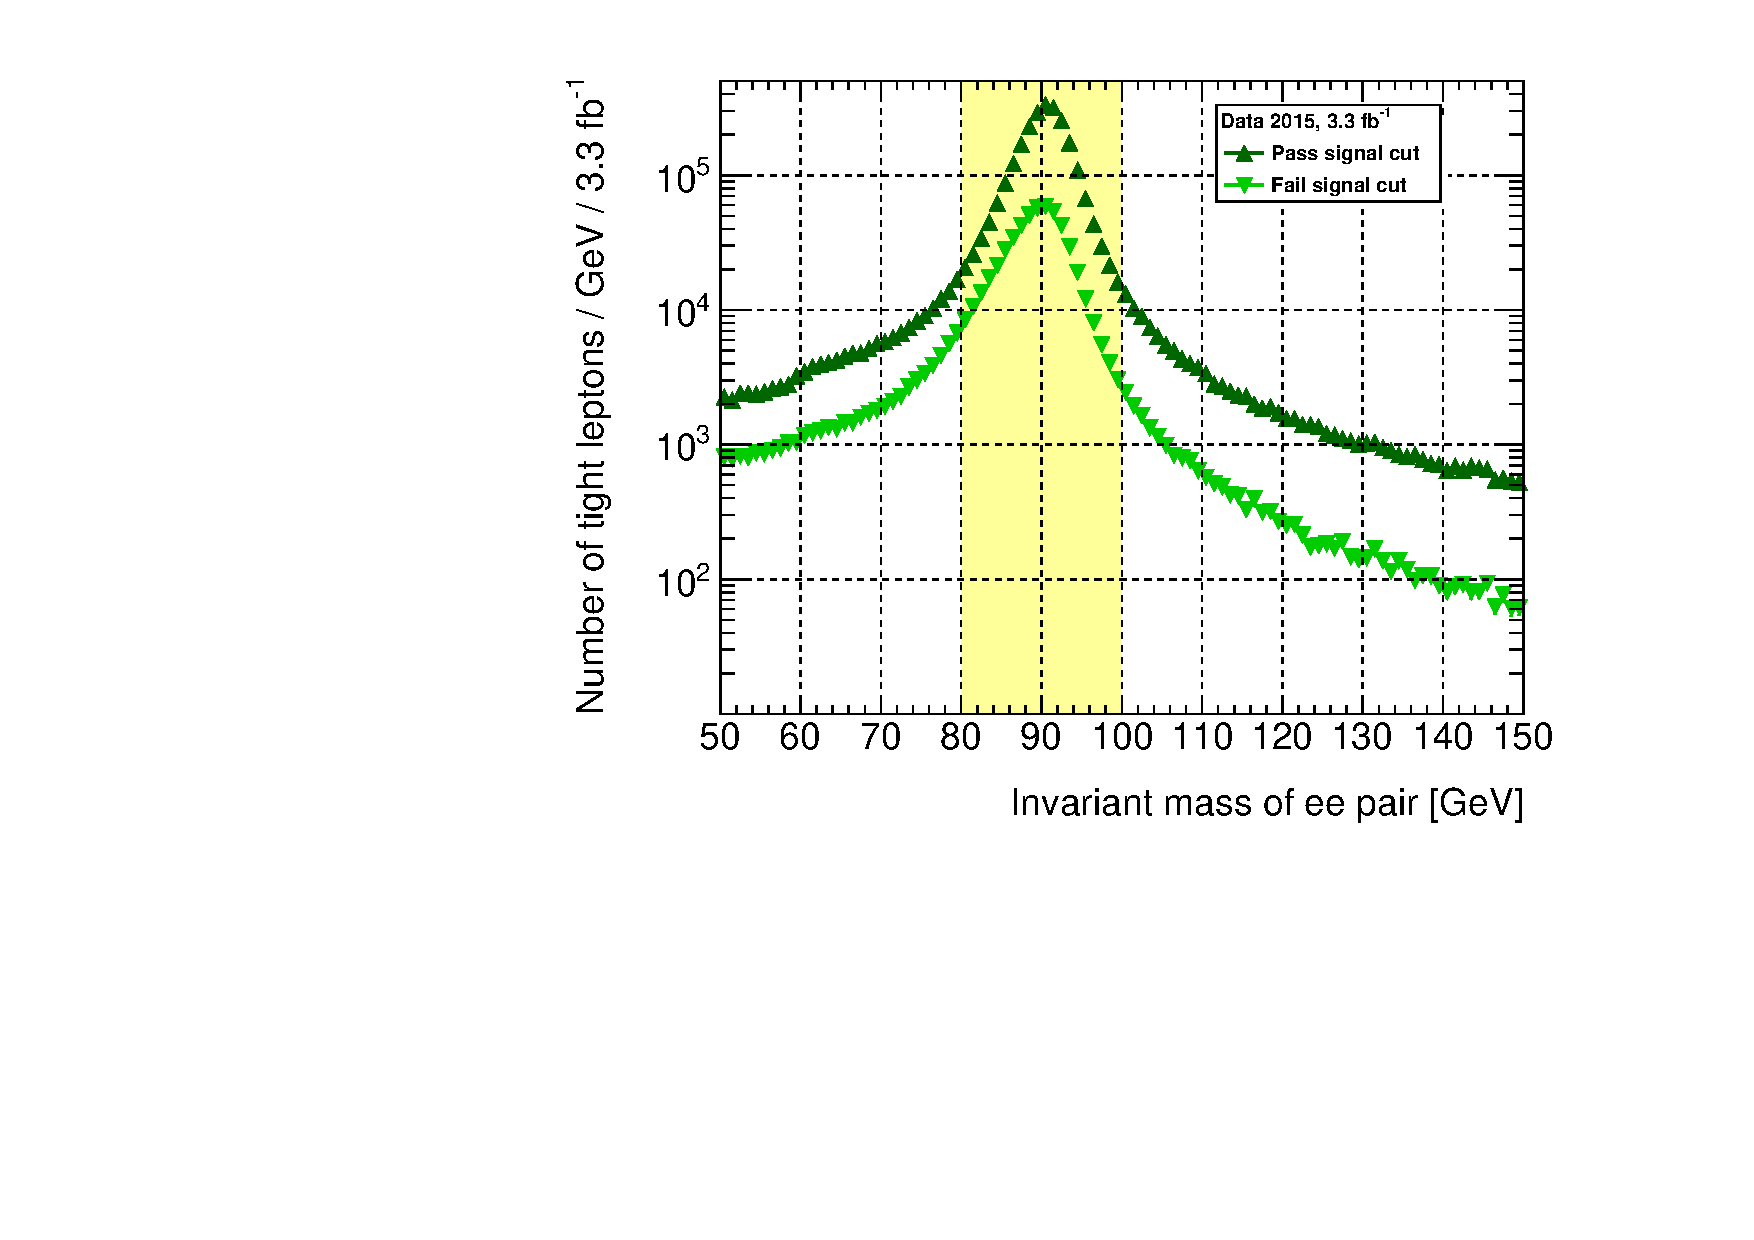
\includegraphics[width=0.45\textwidth]{BKG/realEff/OS_PASSFAIL_EL.pdf}
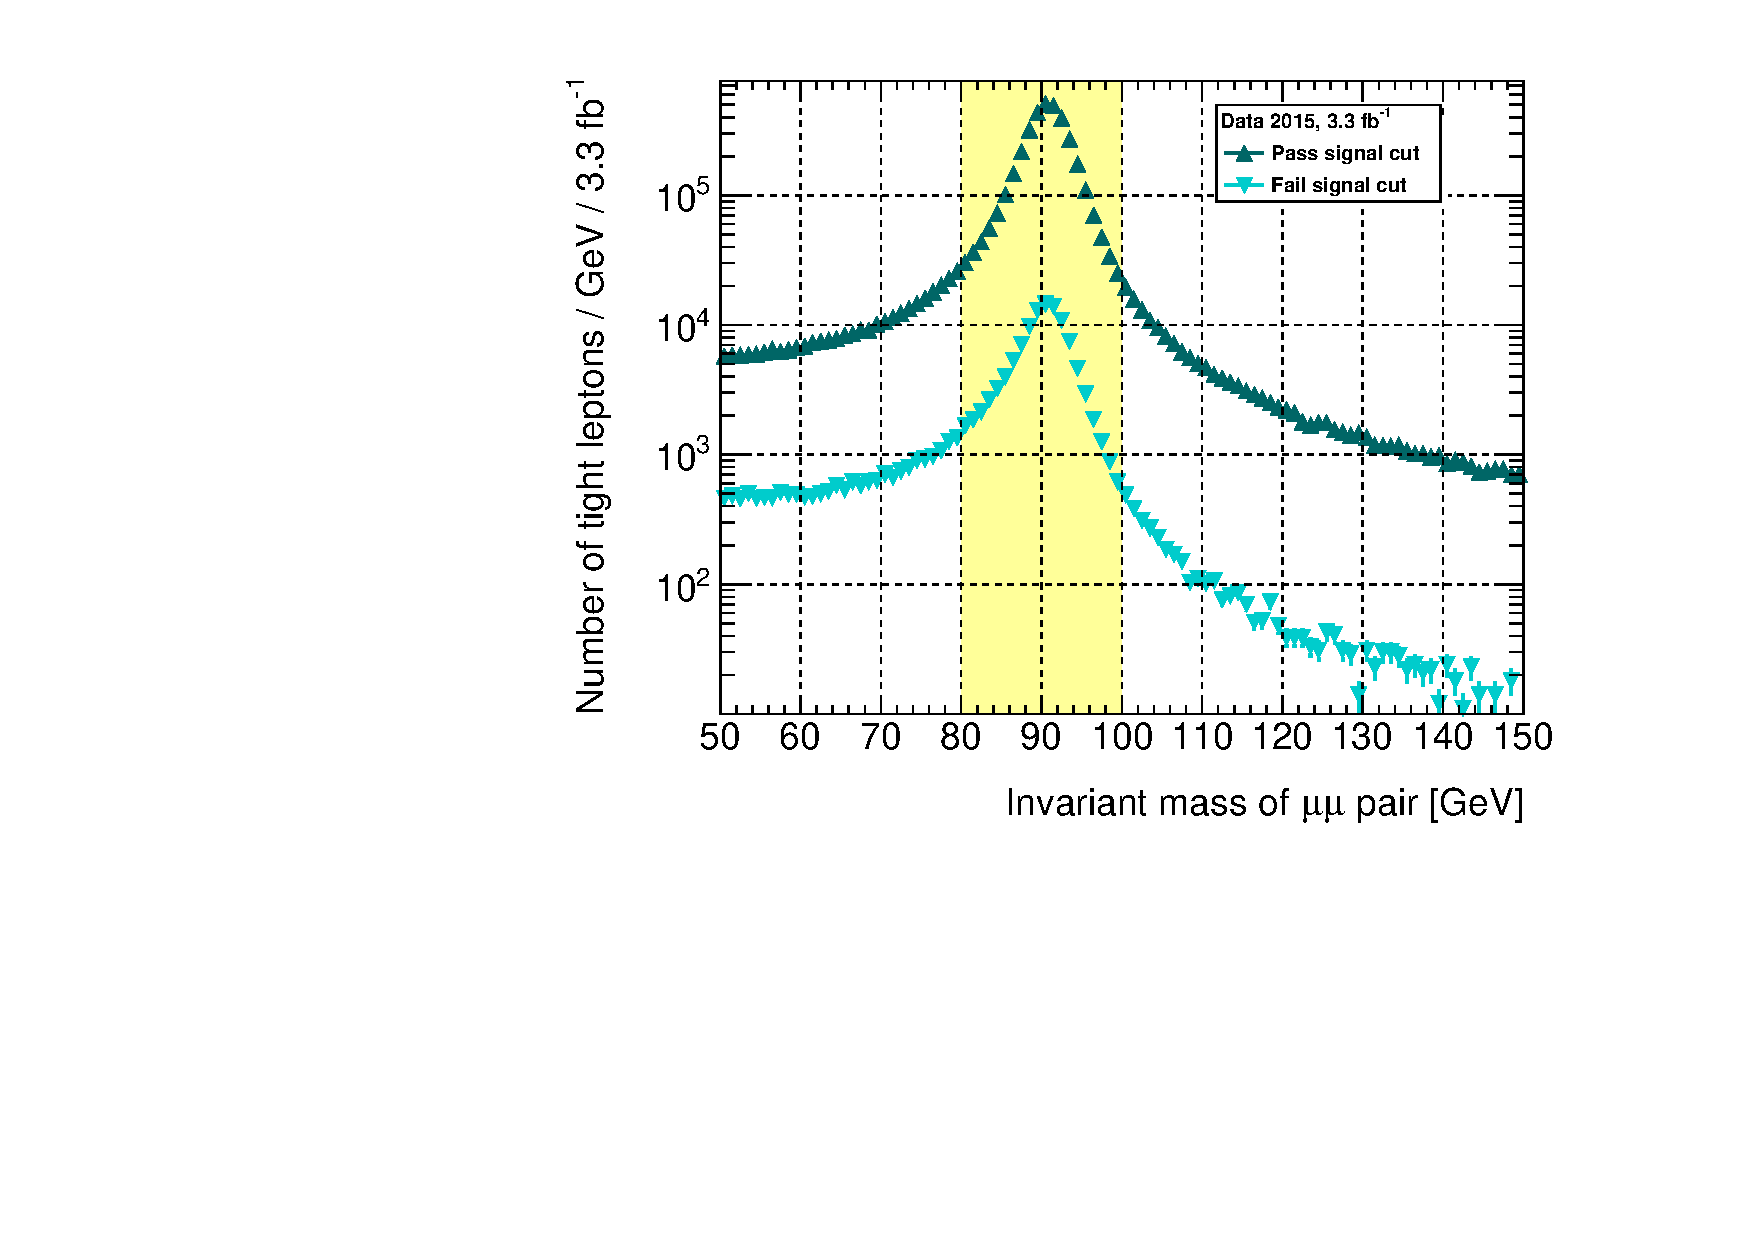
\includegraphics[width=0.45\textwidth]{BKG/realEff/OS_PASSFAIL_MU.pdf}
}
\caption{Invariant mass of the tag-and-probe electron (left) and muon (right) opposite-sign pair, for probes passing/failing the signal requirements. }
\label{Fig:InvMass_realEff}
\end{figure}

A sizable background contamination is observed for the $\pt < 20$ GeV electrons. This contamination is estimated using a background template method inspired by the one used by the $e/\gamma$ CP group to measure reconstruction and identification efficiencies measurements~\cite{ATLAS-CONF-2014-032}. Related systematic uncertainties are set by varying the $m_{ee}$ measurement window and the background template method. Besides, the \texttt{HLT\_2e12\_lhloose\_L12EM10VH} trigger used in the analysis induces a sizable bias to the measurement. As both electrons with and without di-electron trigger match can enter in the signal regions\footnote{If the event is trigger by the di-electron trigger, the two leading electrons are match to the trigger whereas the third one is not. Also, if the event is triggered by the $E_{\mathrm{T}}^{miss}$ trigger the electrons are not match to any triggers.}, a systematic uncertainty is set to cover this effect. As the real muon efficiency is fully dominated by the track isolation cut, the measurement of the track isolation efficiencies performed by the muon CP group using the same $Z$ tag-and-probe technique is very similar. Therefore the systematic uncertainties associated to track isolation efficiency measurement provided by the Muon CP group can be used to assess the systematic uncertainties associated to the muon tag-and-probe measurement method.

A last source of systematic uncertainty is considered to account for the extrapolation from events with well isolated leptons, where the real lepton efficiencies are extracted, to the signal regions characterized by a more busy environment, with several ($b$)-jets. Possible dependencies of the efficiencies to other variables (i.e. $\Delta R(\ell, \text{jet})$, number of jets, etc) have been checked, and the difference with respect to the nominal parametrization is ensured to be within the assigned systematic uncertainty. The opportunity of measuring the efficiencies with a tag-and-probe method based on \ttbar\ events has been studied in order to measure the real lepton efficiencies with events with topology closer to the Signal Regions with leptons close to ($b$)-jets. However, preliminary conclusions shown that the statistics uncertainties associated to this method are too large to perform a measurement with a fine \pt and $\eta$ binning. Therefore we chose to consider this method only when more statistics will be available. More details are given in Appendix~\ref{App:RealEfficiency}. \\


\par{\bf Results\\}
The resulting real efficiencies, measured with the 2015 data at 13 TeV ($3.2~\mathrm{fb}^{-1}$), are shown in Figure~\ref{Fig:Results_realEff}. The electrons efficiencies are dominated by the calorimeter isolation cut at $\pt < 25$ GeV and by the loose to tight likelihood identification cut at $\pt > 25$ GeV. The associated efficiencies increase from $44-70\%$ at low $\pt$ up to $92-94\%$ above 80~GeV. The real muon efficiencies, largely dominated by the track isolation cut, vary from $85\%$ at low $\pt$ to $>95\%$ above 35~GeV. \\
  
\begin{figure}[h!]
\centering
\subfigure{
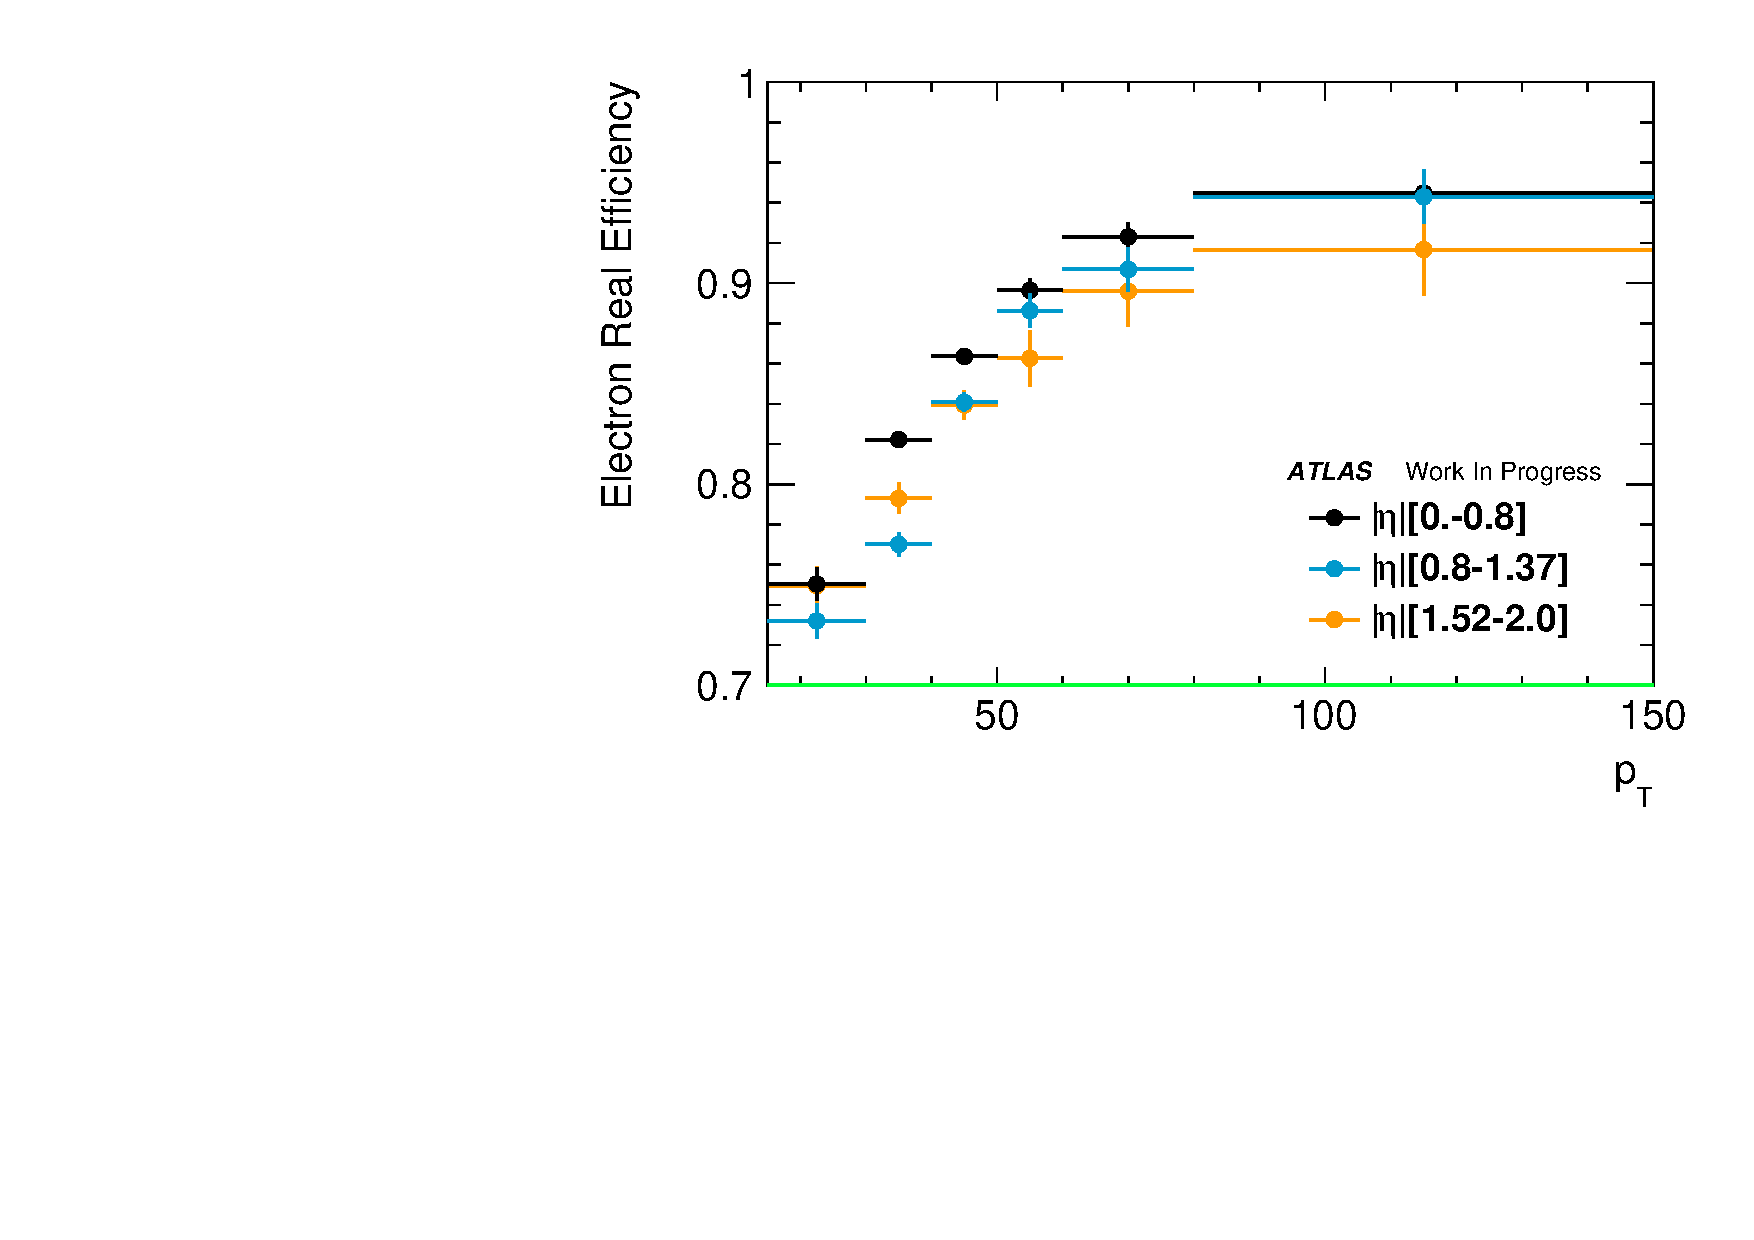
\includegraphics[width=0.45\textwidth]{BKG/realEff/Data_RealEfficiencies_Vs_pt_eta_electrons_ZTandP}
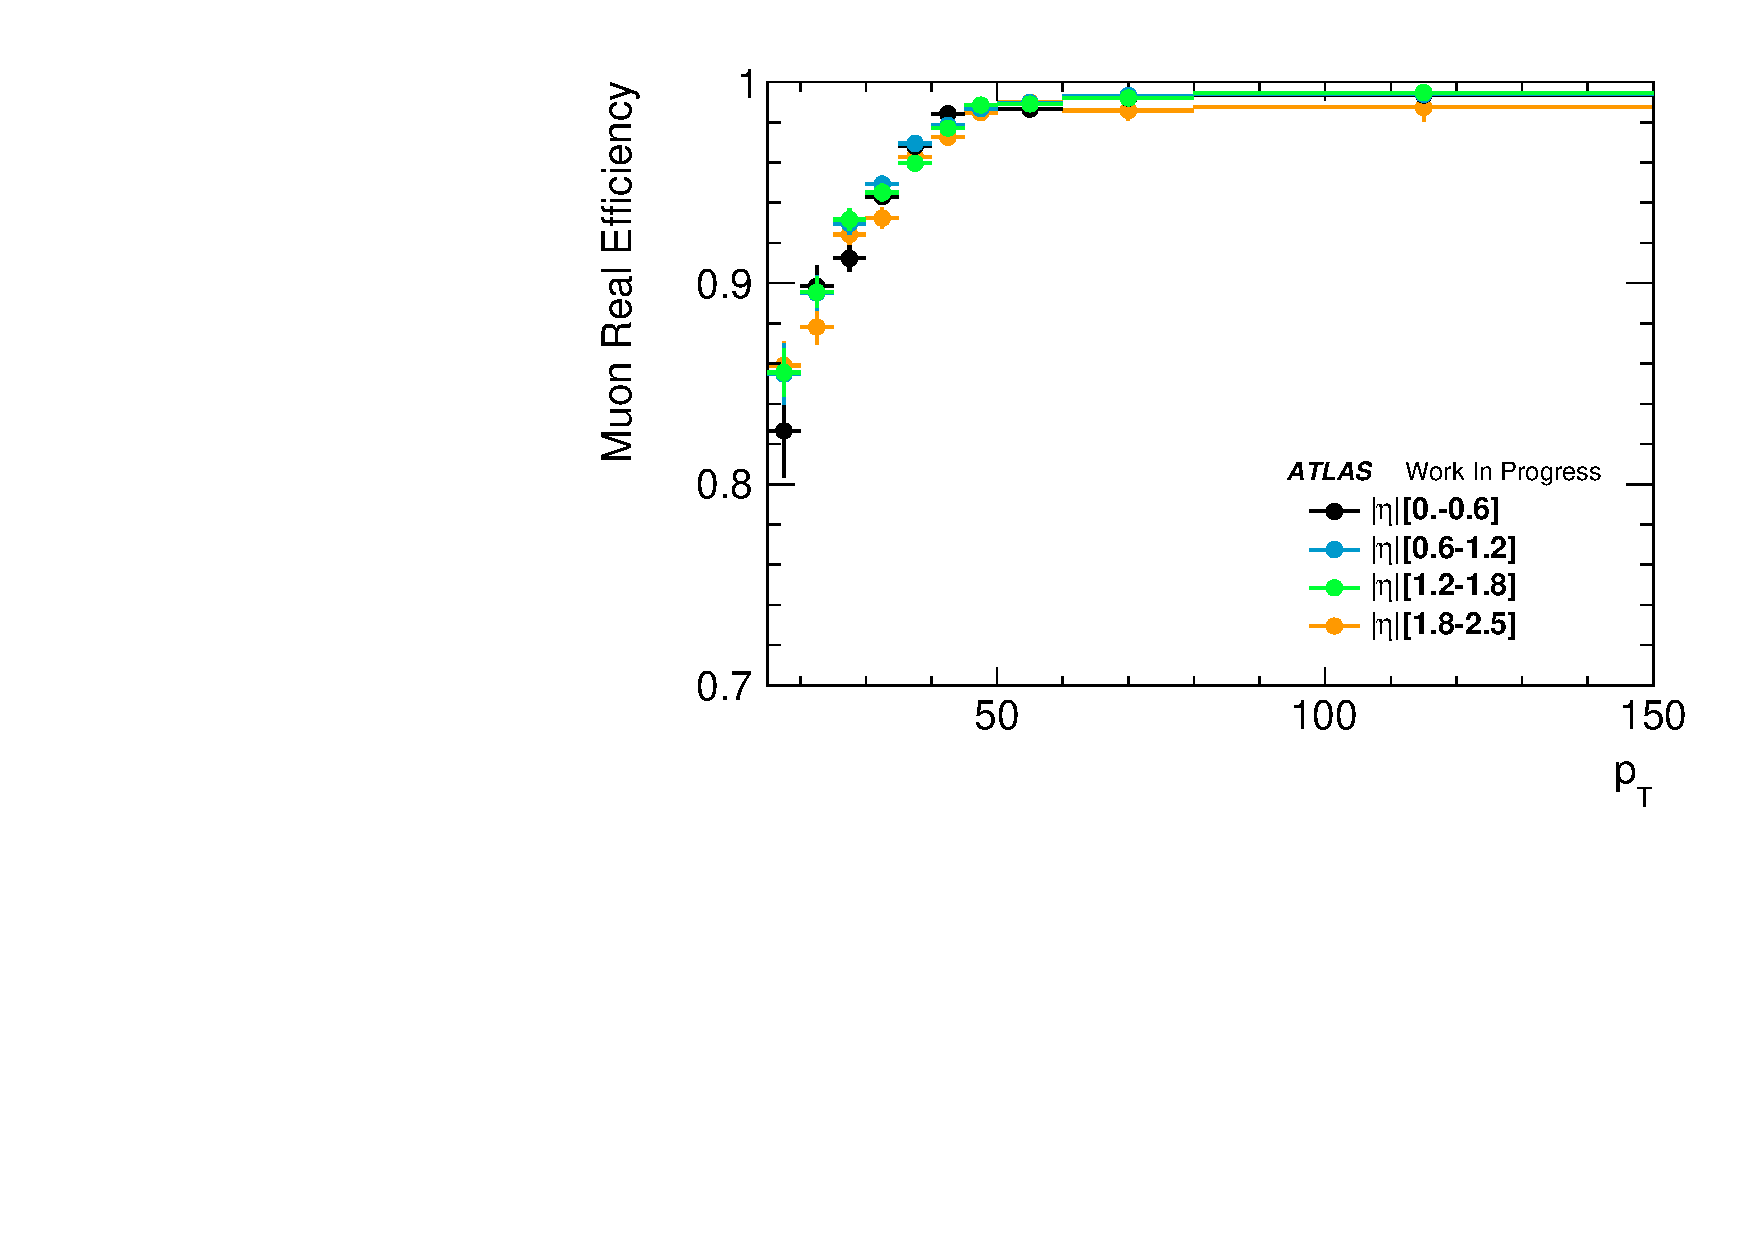
\includegraphics[width=0.45\textwidth]{BKG/realEff/Data_RealEfficiencies_Vs_pt_eta_muons_ZTandP}
}
\vspace{-0.2cm}
\caption{Electron (left) and muon (right) real efficiencies as a function of \pt and $\eta$, in data. The $\eta$ binning used in the electron case corresponds to the geometry of the electromagnetic calorimeter. For muons a homogeneous $\eta$ binning is considered. The error bars corresponds to the quadratic sum of the statistical and tag-and-probe measurement systematic uncertainties.}
\label{Fig:Results_realEff}  
\end{figure}


\par{\bf Systematic uncertainties\\}
Three different sources are considered to assign the systematics uncertainty on the real lepton efficiency: 
\begin{itemize}
	\item Real efficiency measurement : 27 variations of the tag-and-probe method are considered to assess the electron measurement systematics. As done in the $e/\gamma$ CP group~\cite{ATLAS-CONF-2014-032} alternative $m_{ee}$ windows and 9 variations of the background subtraction methods are considered. The largest contribution to the systematics arises from the $m_{ee}$ window variation. This is expected as the proportion of electrons affected by bremsstrahlung depends on $m_{ee}$. The resulting relative systematics vary from $5-7\%$ in the low \pt range to $\sim 0.5\%$ for $\pt >$ 40 GeV. The systematic uncertainties associated to the muon efficiencies measurement vary from $1\%$ in the low \pt range to $O(0.5\%)$ for $\pt >$ 20 GeV.
	\item Di-lepton trigger inefficiency : The bias induced in the real electron efficiency is computed by comparing the efficiency computed with and without trigger match. The resulting relative systematic uncertainty is found to be at most $4\%$ in the $20 < \pt < 35$ GeV range, $2\%$ in the $35 < \pt < 60$ GeV range and $O(0.5\%)$ for electrons in the $\pt > 60$ GeV range.
        \item Extrapolation to signal regions : This systematic is evaluated comparing the real efficiency measured in MC samples for processes such as $Z\to\ell\ell$,~\ttbar\ and a SUSY benchmark model $\tilde{g}\tilde{g} \rightarrow t\overline{t}t\overline{t} \tilde{\chi}^0_1 \tilde{\chi}^0_1$ with $m_{\tilde{g}} - m_{\tilde{\chi}^0_1} > 1000$~GeV. The latter provides an extreme case of boosted tops leading to less well isolated leptons, ensuring that the considered uncertainties are conservative. The corresponding systematics uncertainties, parametrized as a function of the lepton $\pt$ and $\Delta R(\ell,\text{jet})$, are shown in Table~\ref{tab:Real_efficiency_syst}.
\end{itemize}
For both electrons and muons, the statistical uncertainties are found to be negligible with respect to the systematic ones. The signal region extrapolation systematic uncertainties are dominant for muons and electrons close to a jet ($\Delta R(e,\mathrm{jet}) < 0.6$). For electrons with $\Delta R(e,\mathrm{Jet}) > 0.6$, all the systematic uncertainties are at the same order magnitude at low \pt ($\pt < 30$ GeV), while the signal region extrapolation uncertainty dominates in the $\pt > 30$ GeV range. All the systematic are considered as correlated between \pt and $\eta$ bins and more details can be found in Appendix~\ref{App:RealEfficiency}. Despite the large signal region extrapolation systematic uncertainties, the impact of the real lepton efficiencies uncertainties on the estimation of the fake background is marginal with respect to ones from the fake leptons efficiencies.



%%%%%%%%%%%%%%%%%%%%%%%%%%%%%%%%%%%%%%%%%%%%%%%%%%%%%%%%%%%%%
%
\begin{table}[h!]
     \centering
     \begin{tabular}{|l|c|c|}
     \hline
	 \multicolumn{3}{|c|} {\textbf{electrons}}\\
	 \hline 
	 \hline
                 &$0.4 < \Delta R(l,jet) < 0.6$ & $\Delta R(l,jet) > 0.6$\\
	 \hline
	 $\pt < 60$ GeV  &  $8\%$ & $4\%$\\
	 \hline
	 $\pt > 60$ GeV  &  $5\%$  & $5\%$\\
	 \hline		
	 \hline
	 \multicolumn{3}{|c|} {\textbf{muons}} \\  
         \hline
         \hline
                &$0.4 < \Delta R(l,jet) < 0.6$ & $\Delta R(l,jet) > 0.6$\\  
         \hline
         $p_{\mathrm{T}} < 15$ GeV      &    $28\%$    &  $10\%$ \\ 
         \hline
         $15 < p_{\mathrm{T}} < 35$ GeV &    $18\%$    &  $7\%$  \\ 
         \hline
         $35 < p_{\mathrm{T}} < 50$ GeV &    $10\%$    &  $5\%$  \\  
         \hline
         $50 < p_{\mathrm{T}} < 80$ GeV &    $5\%$     &  $3\%$  \\  
         \hline
         $p_{\mathrm{T}} > 80$ GeV      &    $1\%$     &  $1\%$  \\ 
         \hline
         \end{tabular}
\caption{SUSY signal extrapolation systematic uncertainty on the real lepton efficiency measurements.}
\label{tab:Real_efficiency_syst}
\end{table}



%%%%%%%%%%%%%%%%%%%%%%%%%%
\subsubsection{Measurement of the $\zeta$ probabilities (fake leptons)}
\label{sec:FakeRate_DD}

This parameter is measured in dedicated control regions enriched in fake leptons, using a Tag$\&$Probe method. 
Compared to the lepton identification efficiency, the fake lepton efficiency is much harder to determine 
due to the difficulty to identify an event selection that would provide both a high purity and enough statistics, especially for leptons with $\pt>40$~\GeV. 
In the Run-1 (8~\TeV) analysis, the selection was requiring at least two same-sign leptons together with a jet, 
and the fake electron probabilities were determined separately for events with or without $b$-jets. 
Other analyses have been using inclusive selections with a single lepton (dominated by QCD), which have the advantage to be much more populated, but on the other hand are less representative of the properties of fake leptons that can be found in the signal regions. 

A similar approach to Run-1 is used to perform the measurement with the Run-2 data. We select events with two same-sign leptons ($p_T>10$ GeV, satisfying the baseline requirements), one of which (referred to as ``tag'') 
should satisfy the signal requirements and be rather energetic (e.g. $p_T>40$ GeV). For the electron fake rate measurement, the tag should fire (and be matched) to \texttt{HLT\_mu26\_imedium} primary single muon trigger. For the muon fake rate measurement, the events are selected with \texttt{HLT\_mu18\_mu8noL1} di-lepton trigger.
The requirements imposed on the tag allow to enrich the selection in semileptonic $V+$ jets or $t\bar t$ processes with one fake lepton, similar to the signal regions contents, while rejecting QCD events in which the sources of fakes might differ. 
Selected events should also contain at leas one $b$-jet, to enrich the sample in fake leptons from $t\bar t$ processes 
which were seen in MC to dominate the contributions to all signal regions. 
To reduce the contamination in diboson and \ttbar+V processes, any event with a third baseline lepton with \pt~$>$~10~GeV is rejected. The remaining prompt SS background is subtracted using Monte Carlo samples, 
while the charge flip background is subtracted using OS data events re-weighted by the charge flip rate obtained in data, as explained in Section~\ref{sec:bkg_chflips}. To minimize the signal contamination and the overlap with the signal regions, an upper cut of 125~GeV on \met is considered. Finally, the fake rate is measured as the ratio between the number of tight ($N_T$) and tight + loose ($N_T$ + $N_L$) leptons~\footnote{Loose = baseline lepton not passing the signal requirements.}:

\begin{align} 
	\zeta = \frac{N_T-N_T^\text{bkg}}{N_T + N_L -N_T^\text{bkg} -N_L^\text{bkg}},
	\quad (\Delta\zeta)_\text{stat} = \frac 1{N_T+N_L}\sqrt{(1-\zeta)^2 N_T + \zeta^2 N_L}
\end{align}
the latter expression indicates the statistical uncertainty assigned to the measured rate, 
derived with a first order approximation. 

In general the probabilities vary largely with $\pt$ thus require binned measurements. Given the low statistics in data, we chose the performed the measurement only in two \pt bins [10,20]~GeV and $\geq$20~GeV for electrons and three \pt bins for muons ([10,15]~GeV, [15,20]~GeV and $\geq$20~GeV). The dependency on other kinematic variables is studied in $V$+jets and \ttbar\ MC samples, and the difference with respect to nominal measurement is ensured to be within the assigned systematic uncertainty. 

Before showing the actual measurements in data, we present studies based on \ttbar\ and $V$+jets Monte Carlo samples (yielding fake leptons). They provide essentially three important pieces of information: 
\begin{itemize}
\item the nature of the fake lepton sources in the regions used for the data measurements. 
This helped devising regions that have a composition as close as possible to the signal regions (see Section~\ref{sec:truthComposition_SR}) while trying to keep enough statistics for the measurement. 
\item whether, and to which extent, the fake rates differ between the different sources of fake leptons. 
This is a crucial input to define the systematic uncertainties assigned on the measured fake rates and their extrapolation to the signal regions. 
\item how the fake rates depend on various variables related to the topology and the kinematics of the event (lepton $p_T$, number of jets, \met, \meff\ldots)
\end{itemize}
The leptons can be easily identified through truth-matching information, 
therefore the event selections used in these studies are looser than the ones used for the data measurements. 


%%
\par{\bf Nature of the fake leptons\\}
We use $V$ + jets and \ttbar\ MC samples to design a control region enriched in fake leptons that will be further defined in data to measure the lepton fake rates. 
This control region should have a similar composition and sources of fake leptons as the defined signal regions. 
During the optimization studies, it is found that the $W$ and $Z$ + jets processes (with a jet faking an electron) 
can be highly reduced by requiring at least one $b$-jet in the event (CR$_{1bF}$). 
This is illustrated in Figure~\ref{Fig:Fake_Composition_CR} for electrons (top) and muons (bottom). 
The nature of the fake leptons in this control region is shown in Figures~\ref{Fig:truthComposition_ELFR_CR}~-~\ref{Fig:truthComposition_MUFR_CR}, top. 
For completeness, Figures~\ref{Fig:truthComposition_ELFR_CR}~-~\ref{Fig:truthComposition_MUFR_CR} (bottom) 
show also the origin of fake leptons in a control region region with at least 2 $b$-jets (CR$_{2bF}$). 
The latter is used to examine the difference between the nominal fake rate (measured in CR$_{1bF}$) 
and the fake rate representative for regions with at least two $b$-jets in the event (and measured in CR$_{2bF}$). 
Generally, a similar origin of the fake leptons as in the signal regions is obtained. 

\begin{figure}[h!]
\centering
\subfigure{
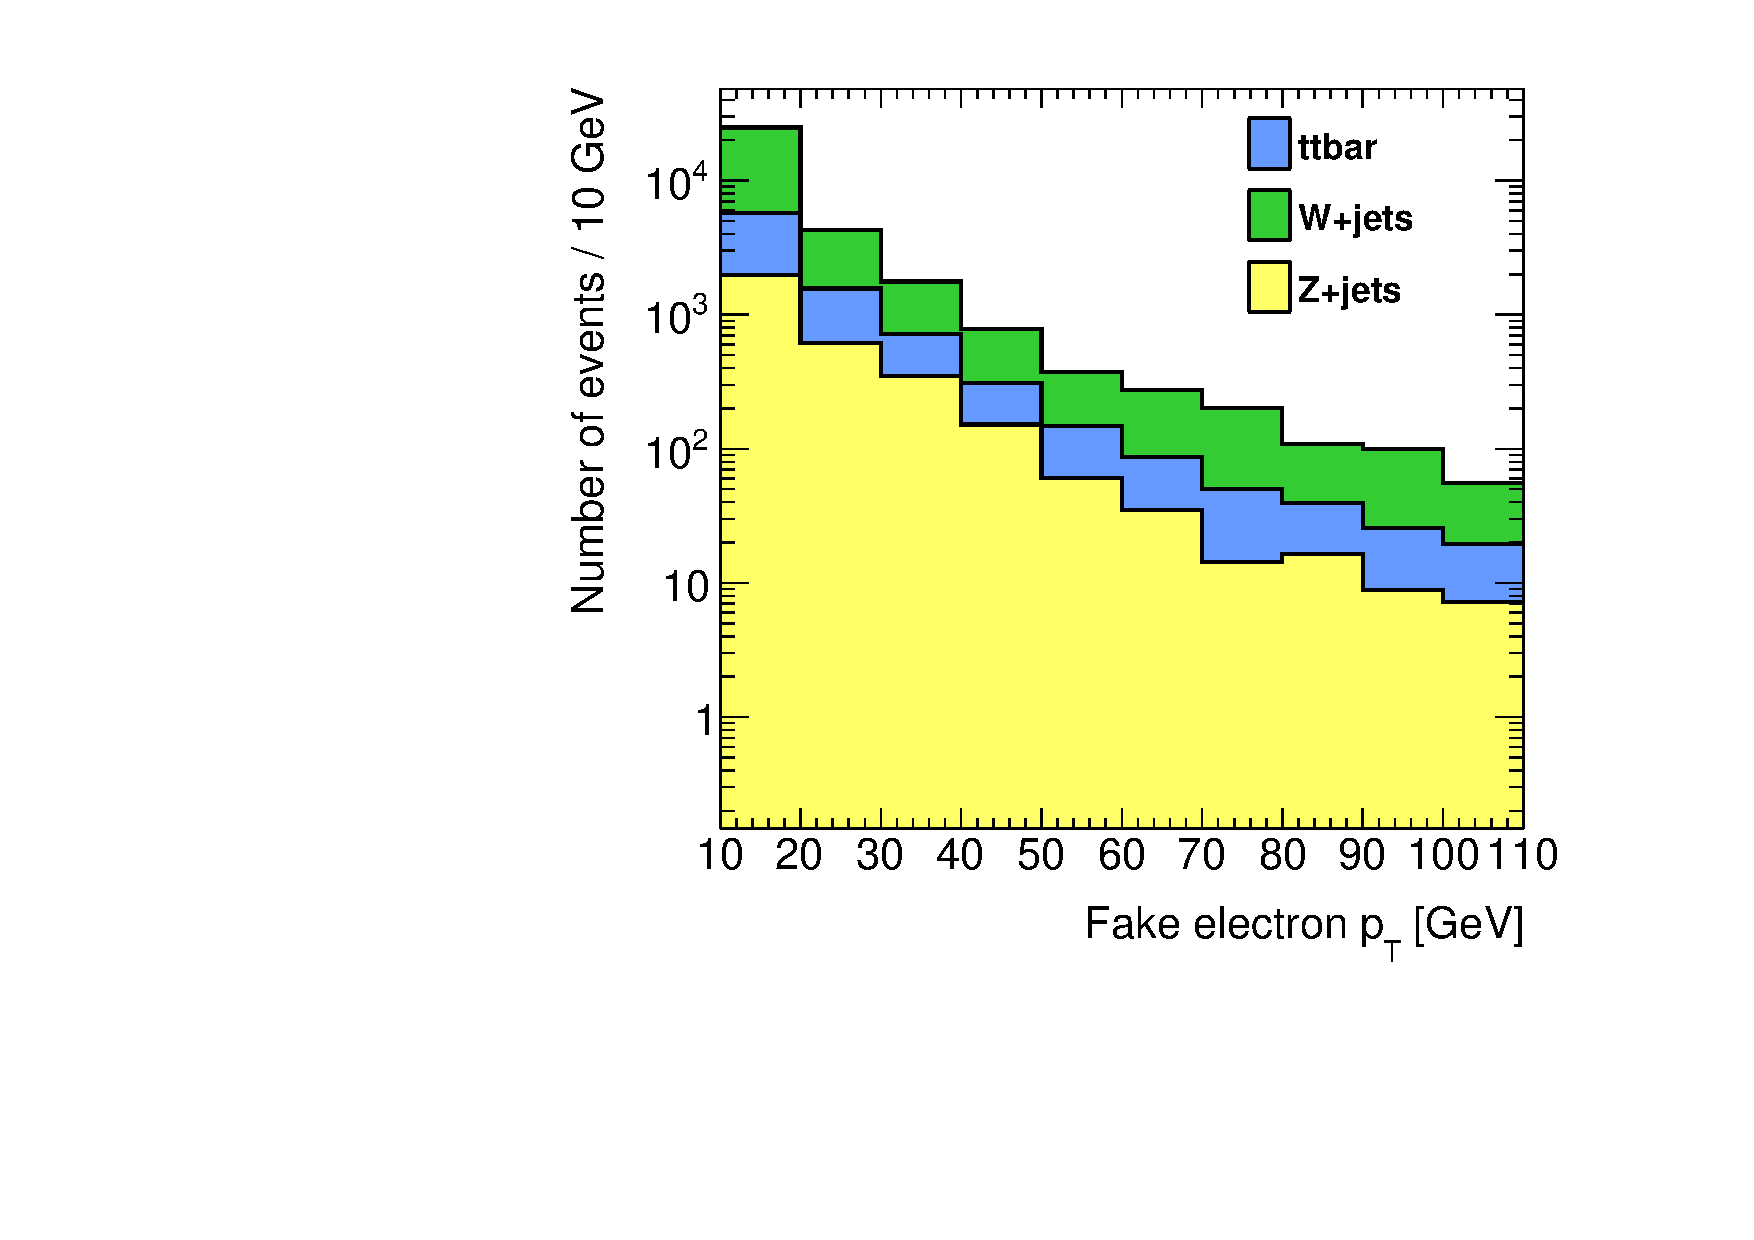
\includegraphics[width=0.45\textwidth]{FIGURES/Truth_Composition/FakeRate_CR/BaseEL_CRAllPt}
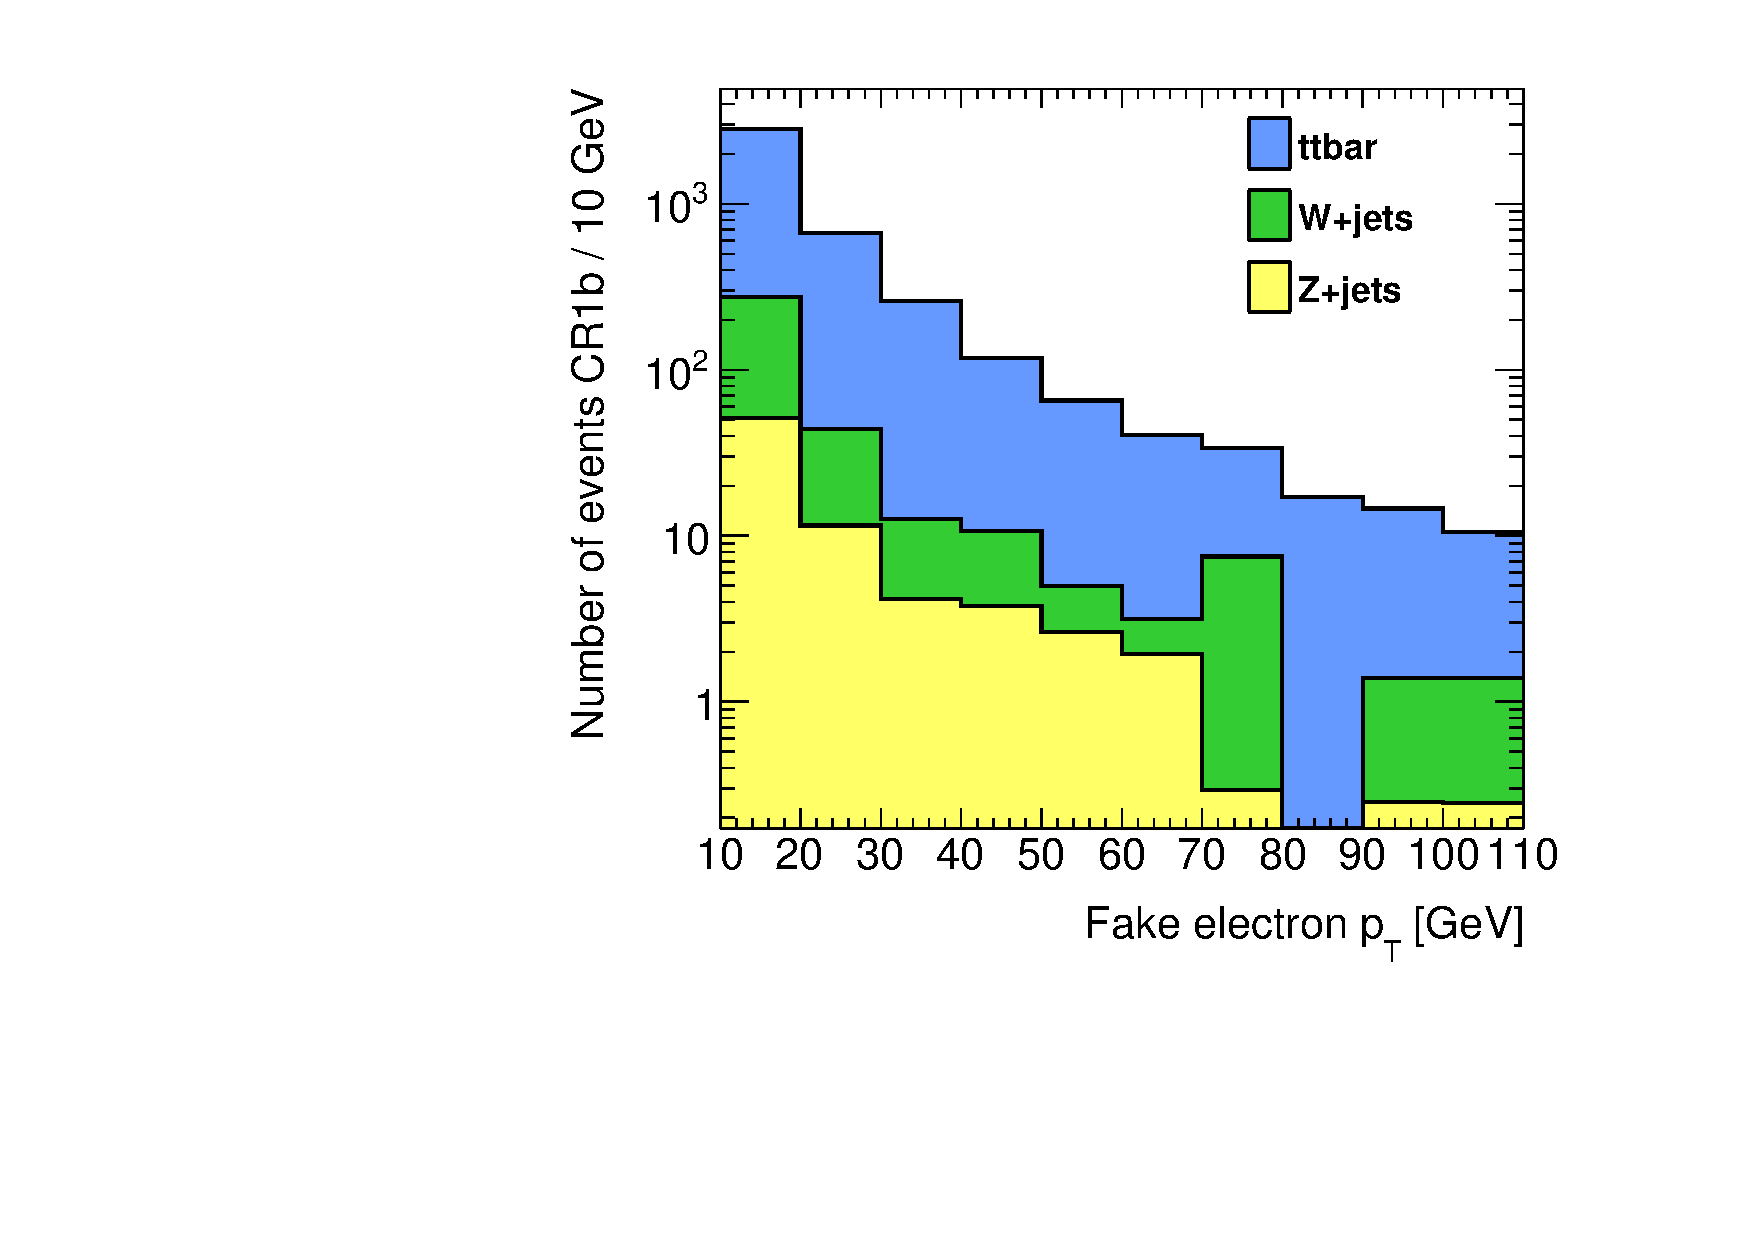
\includegraphics[width=0.45\textwidth]{FIGURES/Truth_Composition/FakeRate_CR/BaseEL_CR1bPt}
}
\subfigure{
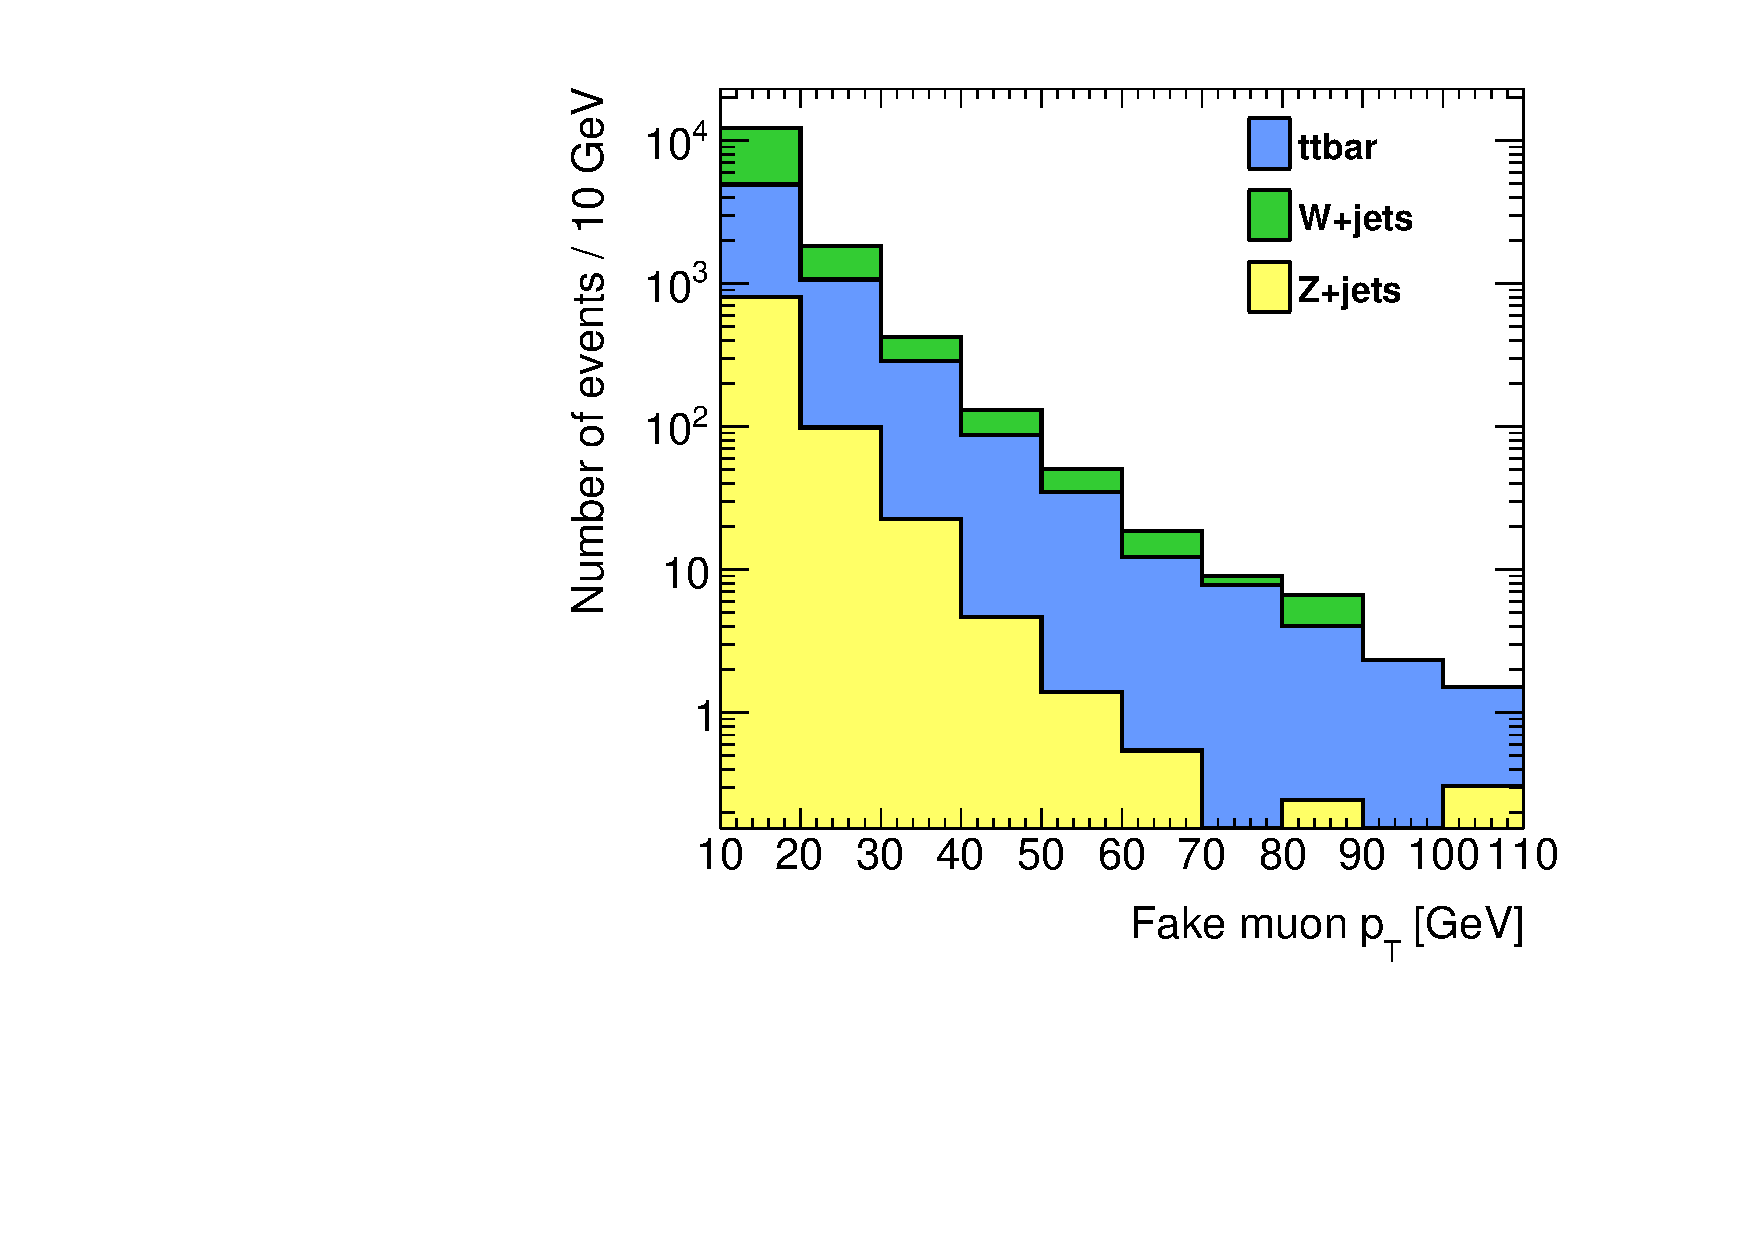
\includegraphics[width=0.45\textwidth]{FIGURES/Truth_Composition/FakeRate_CR/BaseMU_CRAllPt}
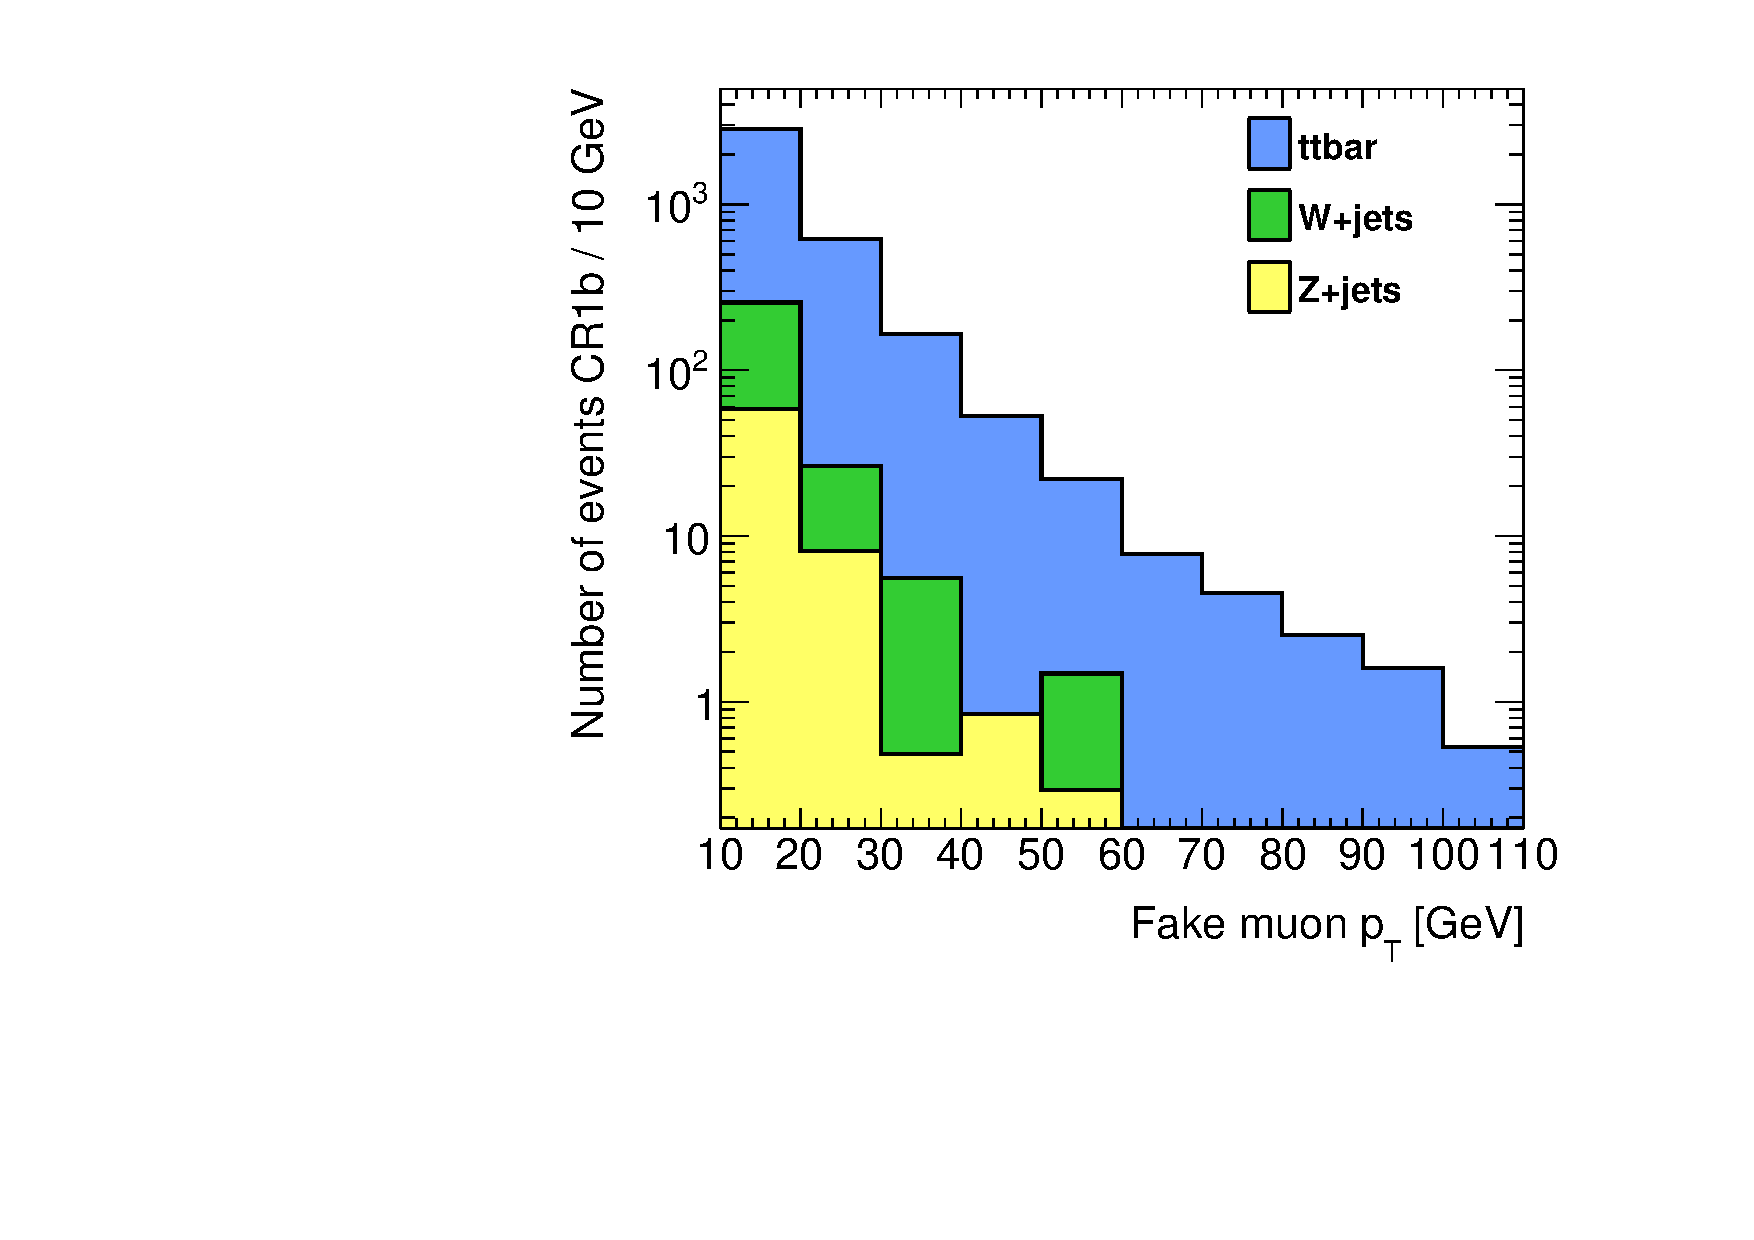
\includegraphics[width=0.45\textwidth]{FIGURES/Truth_Composition/FakeRate_CR/BaseMU_CR1bPt}
}
\vspace{-0.2cm}
\caption{Transverse momentum distribution of the fake electrons as predicted by MC simulations after the baseline lepton selection (left) and after requiring at least one $b$-jet in the event (right). Fake electrons (top) and muons (bottom) originating from $t\bar t$ or $V+$ jets events are distinguished. $L$~=~3~\ifb.}
\label{Fig:Fake_Composition_CR}  
\end{figure}
 %%
\begin{figure}[h!]
\centering
\subfigure[Baseline electrons, CR$_{1bF}$] 
{\includegraphics[width=0.49\textwidth]{Truth_Composition/FakeRate_CR/baseline/Vj_1EL_pT_Var_DEF2}}
\subfigure[Signal electrons, CR$_{1bF}$]{
\includegraphics[width=0.49\textwidth]{Truth_Composition/FakeRate_CR/signal/Vj_1EL_pT_Var_DEF2}
}
\subfigure[Baseline electrons, CR$_{2bF}$]
{\includegraphics[width=0.49\textwidth]{Truth_Composition/FakeRate_CR/baseline/Vj_1EL_pT_Var_DEF6.pdf}}
\subfigure[Signal electrons, CR$_{2bF}$]{
\includegraphics[width=0.49\textwidth]{Truth_Composition/FakeRate_CR/signal/Vj_1EL_pT_Var_DEF6.pdf}
}
\caption
{Sources of fake electron as a function of the electron $p_T$, as predicted by MC simulations (combined $t\bar t$ and $V+$ jets) in CR$_{1bF}$ (top) and CR$_{2bF}$ (bottom). The results are shown for baseline (left) or signal electrons (right).} 
\label{Fig:truthComposition_ELFR_CR}
\end{figure}
%%
\begin{figure}[h!]
\centering
\subfigure[Baseline muons, CR$_{1bF}$] 
{\includegraphics[width=0.49\textwidth]{Truth_Composition/FakeRate_CR/baseline/Vj_1MU_pT_Var_DEF2}}
\subfigure[Signal muons, CR$_{1bF}$]{
\includegraphics[width=0.49\textwidth]{Truth_Composition/FakeRate_CR/signal/Vj_1MU_pT_Var_DEF2}
}
\subfigure[Baseline muons, CR$_{2bF}$]
{\includegraphics[width=0.49\textwidth]{Truth_Composition/FakeRate_CR/baseline/Vj_1MU_pT_Var_DEF6.pdf}}
\subfigure[Signal muons, CR$_{2bF}$]{
\includegraphics[width=0.49\textwidth]{Truth_Composition/FakeRate_CR/signal/Vj_1MU_pT_Var_DEF6.pdf}
}
\caption
{Sources of fake muons as a function of the muon $p_T$, as predicted by MC simulations (combined $t\bar t$ and $V+$ jets) in CR$_{1bF}$ (top) and CR$_{2bF}$ (bottom). The results are shown for baseline (left) or signal muons (right).} 
\label{Fig:truthComposition_MUFR_CR}  
\end{figure}
%%


%%
\par{\bf Fake lepton rate in $V$ + jets and in \ttbar\ MC\\}
In this paragraph we present the fake rate measured separately for different sources of fake leptons in $V$ + jets and \ttbar\ MC. 
The truth classification presented in~\ref{sec:truth_matching} is employed to build the different categories. No cut on number of $b$-jets or light jets is applied.

Figure~\ref{Fig:Vjets_FR_ELE} presents the fake rate for electrons arising from hadron decays (light flavor), 
non-prompt electrons (heavy flavor) and converted prompt photons, in $V$+jets MC sample. 
For completeness we also show separately the fake rate for electrons arising from $b$-mesons and $c$-mesons decays. 
Results in \ttbar\ MC are shown in figure~\ref{Fig:TTBAR_FR_ELE}. 
Generally the fake rate is highly dependent on the origin of the fake lepton. 
Thus, it is very important to design at best a control region with a similar composition as the signal regions 
to perform the measurement of the fake rate. 
The fake rates measured in $V$ + jets and in \ttbar\ MC samples differ by a factor greater than 2 in the low \pt range 
for non-prompt electrons, the dominant source in the (relaxed) signal regions.

%%
\begin{figure}[p!]
\centering
\subfigure[Electrons, all sources] 
{\includegraphics[width=0.49\textwidth]{BKG/fakeEff/FakeRate_MC/Only_Vjets/Var0_FakeEL_Reg_Incl_EM_EE_pt}}
\subfigure[Electrons, hadron decays]{
\includegraphics[width=0.49\textwidth]{BKG/fakeEff/FakeRate_MC/Only_Vjets/LightFL/Var0_FakeEL_Reg_Incl_EM_EE_pt}
}
\subfigure[Electrons, converted prompt photons]
{\includegraphics[width=0.49\textwidth]{BKG/fakeEff/FakeRate_MC/Only_Vjets/ConvFL/Var0_FakeEL_Reg_Incl_EM_EE_pt}}
\subfigure[Non-prompt electrons]{
\includegraphics[width=0.49\textwidth]{BKG/fakeEff/FakeRate_MC/Only_Vjets/HeavyFL/Var0_FakeEL_Reg_Incl_EM_EE_pt}
}
\subfigure[Electrons, $b$-mesons decays]
{\includegraphics[width=0.49\textwidth]{BKG/fakeEff/FakeRate_MC/Only_Vjets/BFL/Var0_FakeEL_Reg_Incl_EM_EE_pt}}
\subfigure[Electrons, $c$-mesons decays]{
\includegraphics[width=0.49\textwidth]{BKG/fakeEff/FakeRate_MC/Only_Vjets/CFL/Var0_FakeEL_Reg_Incl_EM_EE_pt}
}
\caption
{Electron fake rate in $V$+jets MC sample. Results are shown separately for different sources of fake electrons.} 
\label{Fig:Vjets_FR_ELE}  
\end{figure}
%%
\begin{figure}[p!]
\centering
\subfigure[Electrons, all sources] 
{\includegraphics[width=0.49\textwidth]{BKG/fakeEff/FakeRate_MC/Only_ttBar/Var0_FakeEL_Reg_Incl_EM_EE_pt}}
\subfigure[Electrons, hadron decays]{
\includegraphics[width=0.49\textwidth]{BKG/fakeEff/FakeRate_MC/Only_ttBar/LightFL/Var0_FakeEL_Reg_Incl_EM_EE_pt}
}
\subfigure[Electrons, converted prompt photons]
{\includegraphics[width=0.49\textwidth]{BKG/fakeEff/FakeRate_MC/Only_ttBar/ConvFL/Var0_FakeEL_Reg_Incl_EM_EE_pt}}
\subfigure[Non-prompt electrons]{
\includegraphics[width=0.49\textwidth]{BKG/fakeEff/FakeRate_MC/Only_ttBar/HeavyFL/Var0_FakeEL_Reg_Incl_EM_EE_pt}
}
\subfigure[Electrons, $b$-mesons decays]
{\includegraphics[width=0.49\textwidth]{BKG/fakeEff/FakeRate_MC/Only_ttBar/BFL/Var0_FakeEL_Reg_Incl_EM_EE_pt}}
\subfigure[Electrons, $c$-mesons decays]{
\includegraphics[width=0.49\textwidth]{BKG/fakeEff/FakeRate_MC/Only_ttBar/CFL/Var0_FakeEL_Reg_Incl_EM_EE_pt}
}
\caption
{Electron fake rate in \ttbar\ MC sample. Results are shown separately for different sources of fake electrons.} 
\label{Fig:TTBAR_FR_ELE}  
\end{figure}
%%


Figure~\ref{Fig:Vjets_FR_MU} presents the fake rate for muons arising from hadron decays (light flavor) and for non-prompt muons (heavy flavor), in $V$+jets MC sample. 
For completeness we also show separately the fake rate for muons arising from $b$-mesons and $c$-mesons decays. 
Results in \ttbar\ MC are shown in figure~\ref{Fig:TTBAR_FR_MU}. 
The fake rate measured in a region dominated by muons arising from $c$-mesons decays from $V$+jets (in particular from $W$+jets) is up to 50\% higher 
than the fake rate measured in a region dominated by $c$-mesons sources from \ttbar. 
This is mainly because in \ttbar\ the fake muon actually comes from processes like $B\to cX$, hence they are less isolated. 
The $W$+jets processes are not contributing significantly in any of the signal regions, 
thus the fake rate is not additionally measured in a region dominated by such processes. 

%%
\begin{figure}[p!]
\centering
\subfigure[Muons, all sources] 
{\includegraphics[width=0.49\textwidth]{BKG/fakeEff/FakeRate_MC/Only_Vjets/Var0_FakeMU_Reg_Incl_EM_MM_pt}}
\subfigure[Muons, hadron decays]{
\includegraphics[width=0.49\textwidth]{BKG/fakeEff/FakeRate_MC/Only_Vjets/LightFL/Var0_FakeMU_Reg_Incl_EM_MM_pt}
}
\subfigure[Non-prompt muons]{
\includegraphics[width=0.49\textwidth]{BKG/fakeEff/FakeRate_MC/Only_Vjets/HeavyFL/Var0_FakeMU_Reg_Incl_EM_MM_pt}
}
\subfigure[Muons, $b$-mesons decays]
{\includegraphics[width=0.49\textwidth]{BKG/fakeEff/FakeRate_MC/Only_Vjets/BFL/Var0_FakeMU_Reg_Incl_EM_MM_pt}}
\subfigure[Muons, $c$-mesons decays]{
\includegraphics[width=0.49\textwidth]{BKG/fakeEff/FakeRate_MC/Only_Vjets/CFL/Var0_FakeMU_Reg_Incl_EM_MM_pt}
}
\caption
{Muon fake rate in $V$+jets MC sample. Results are shown separately for different sources of fake muons.} 
\label{Fig:Vjets_FR_MU}  
\end{figure}
%%
\begin{figure}[p!]
\centering
\subfigure[Muons, all sources] 
{\includegraphics[width=0.49\textwidth]{BKG/fakeEff/FakeRate_MC/Only_ttBar/Var0_FakeMU_Reg_Incl_EM_MM_pt}}
\subfigure[Muons, hadron decays]{
\includegraphics[width=0.49\textwidth]{BKG/fakeEff/FakeRate_MC/Only_ttBar/LightFL/Var0_FakeMU_Reg_Incl_EM_MM_pt}
}
\subfigure[Non-prompt muons]{ 
\includegraphics[width=0.49\textwidth]{BKG/fakeEff/FakeRate_MC/Only_ttBar/HeavyFL/Var0_FakeMU_Reg_Incl_EM_MM_pt}
}
\subfigure[Muons, $b$-mesons decays]
{\includegraphics[width=0.49\textwidth]{BKG/fakeEff/FakeRate_MC/Only_ttBar/BFL/Var0_FakeMU_Reg_Incl_EM_MM_pt}}
\subfigure[Muons, $c$-mesons decays]{
\includegraphics[width=0.49\textwidth]{BKG/fakeEff/FakeRate_MC/Only_ttBar/CFL/Var0_FakeMU_Reg_Incl_EM_MM_pt}
}
\caption
{Muon fake rate in \ttbar\ MC sample. Results are shown separately for different sources of fake muons.} 
\label{Fig:TTBAR_FR_MU}  
\end{figure}
%%

%%
\par{\bf Fake lepton rate in $W\gamma$ MC\\}
The $W\gamma$ yields close-to and in the SRs are studied by comparing the contribution between $W\gamma$ and other processes using Monte Carlo prediction.
This study shows negligible contribution from $W\gamma$ processes in all SRs.
Compared to other sources leading to fake leptons, Wgamma contributes less than 1\% in regions close-to SR1b and SR3b.
As the electron fake rate is highly dependent on the fake lepton sources, we measure the fake rate also in Wgamma MC samples. 
This allows us to quantify the difference between the nominal fake rate used in the analysis and the fake rate corresponding to photon conversion sources. 
A fake rate around 9\% is obtained. Considering the small contribution and compatible fake efficiency, the $W\gamma$ process could be ignored in the fake rate measurement.

%%
\par{\bf Fake electron efficiency measurement\\}
As the $ee$ channel is dominated by charge flip electrons, the measurement in data is performed using $e\mu$ pairs 
in which the muon is considered to be the tag lepton. 
The numbers of events with tight and loose probe electrons used for the measurement are shown in Table~\ref{table:fake_electron_bjet} 
for data and for Monte Carlo (which are used for the prompt SS subtraction). 
For illustration, Figure~\ref{Fig:CR_fake_ele} shows the $p_T$ distribution of numerator and denominator in data and MC. 
Forcompletness, we choose to show the detector background sources from \ttbar\ and $V$+jets (here the charge-flip is estimated from \ttbar). 
One can see that the MC prediction agrees rather well with data, and the selection is fully dominated by $t\bar t$ processes, as targeted. 
The measured electron fake rates (with their statistical uncertainties) in data, and in $V$+jets and \ttbar\ MC are shown in Table~\ref{table:fake_electron_bjet_Data_MC}. 
The fake rate in data, in the second \pt bin is found to be larger than in MC. This difference is within the assigned systematic uncertainties. 

%%
\begin{figure}[h!]
\centering
\subfigure[CR$_{1bF}$, baseline probe electron]
{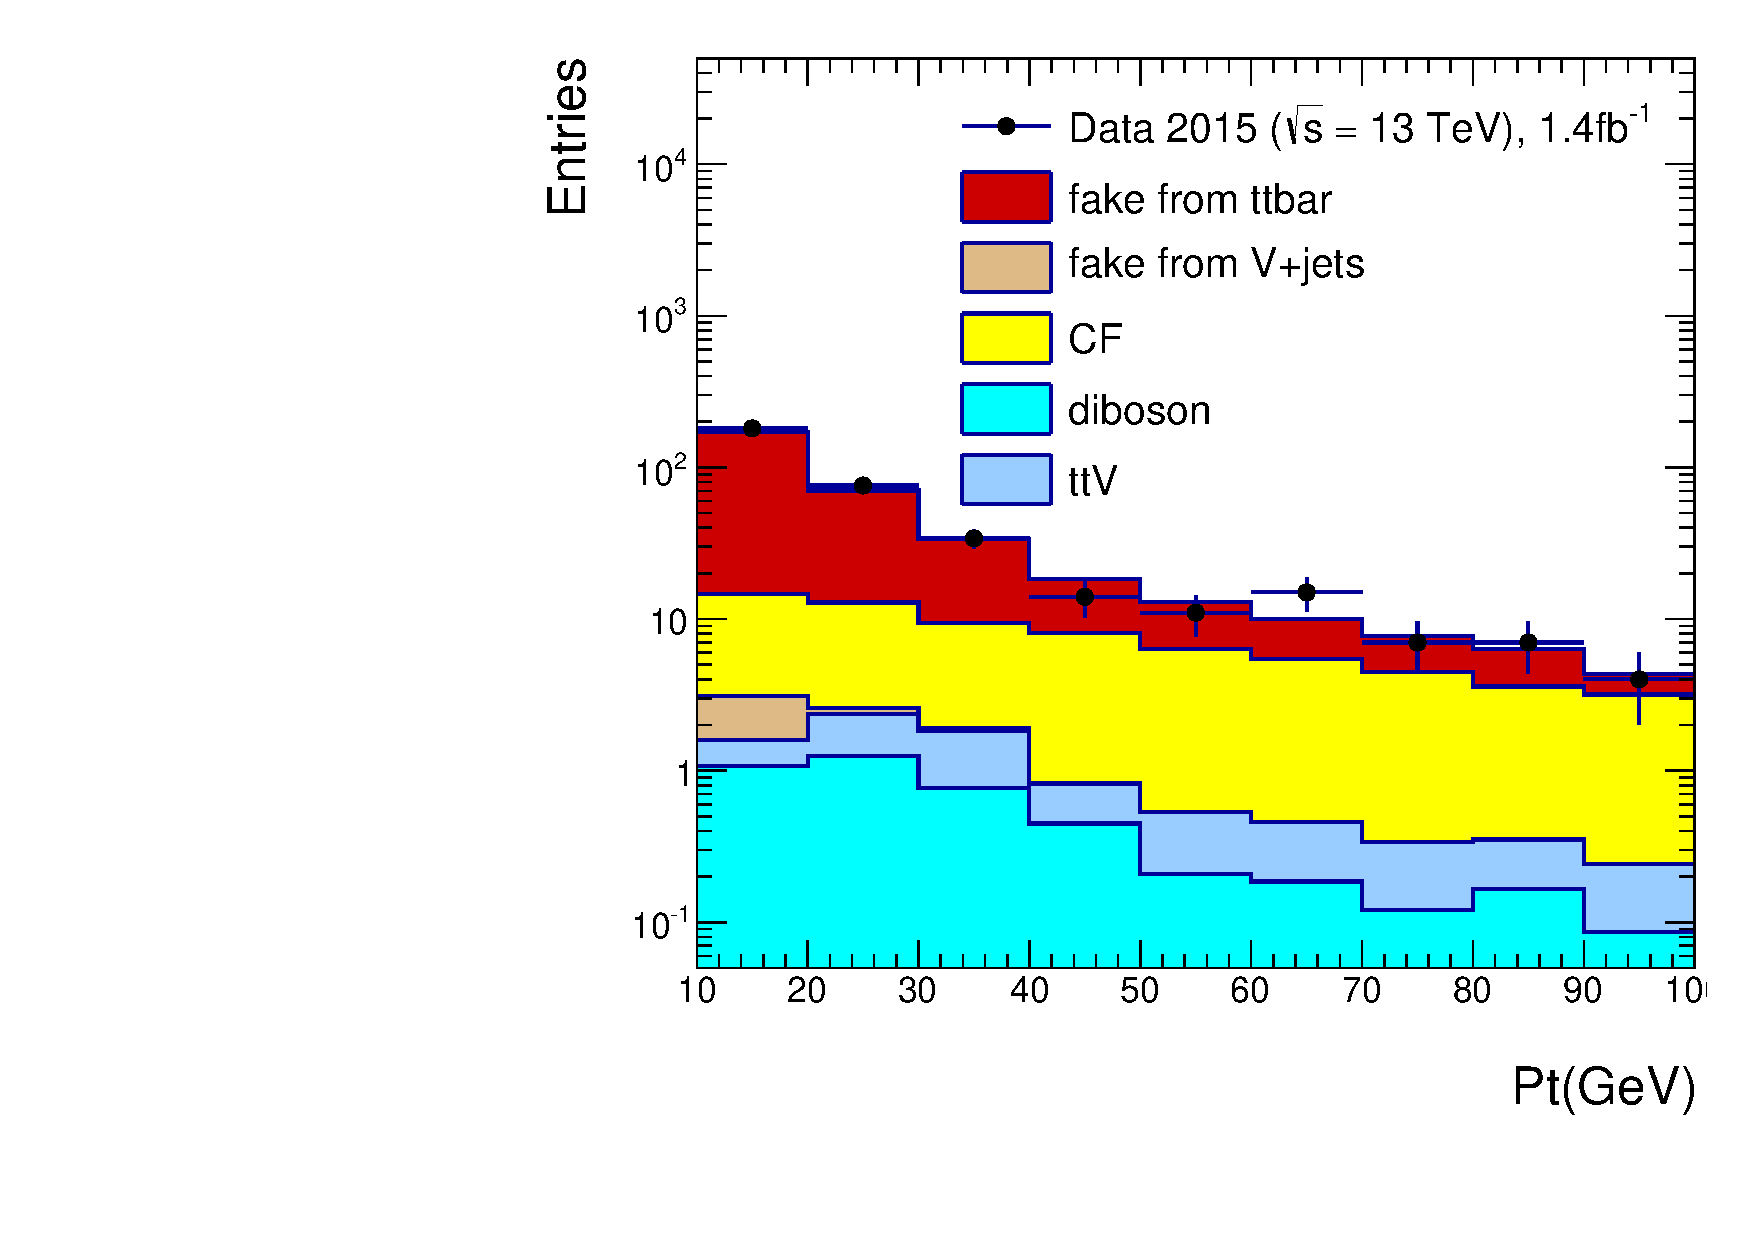
\includegraphics[width=0.49\textwidth]{BKG/fakeEff/el_baseline.pdf}}
\subfigure[CR$_{1bF}$, signal probe electron]{
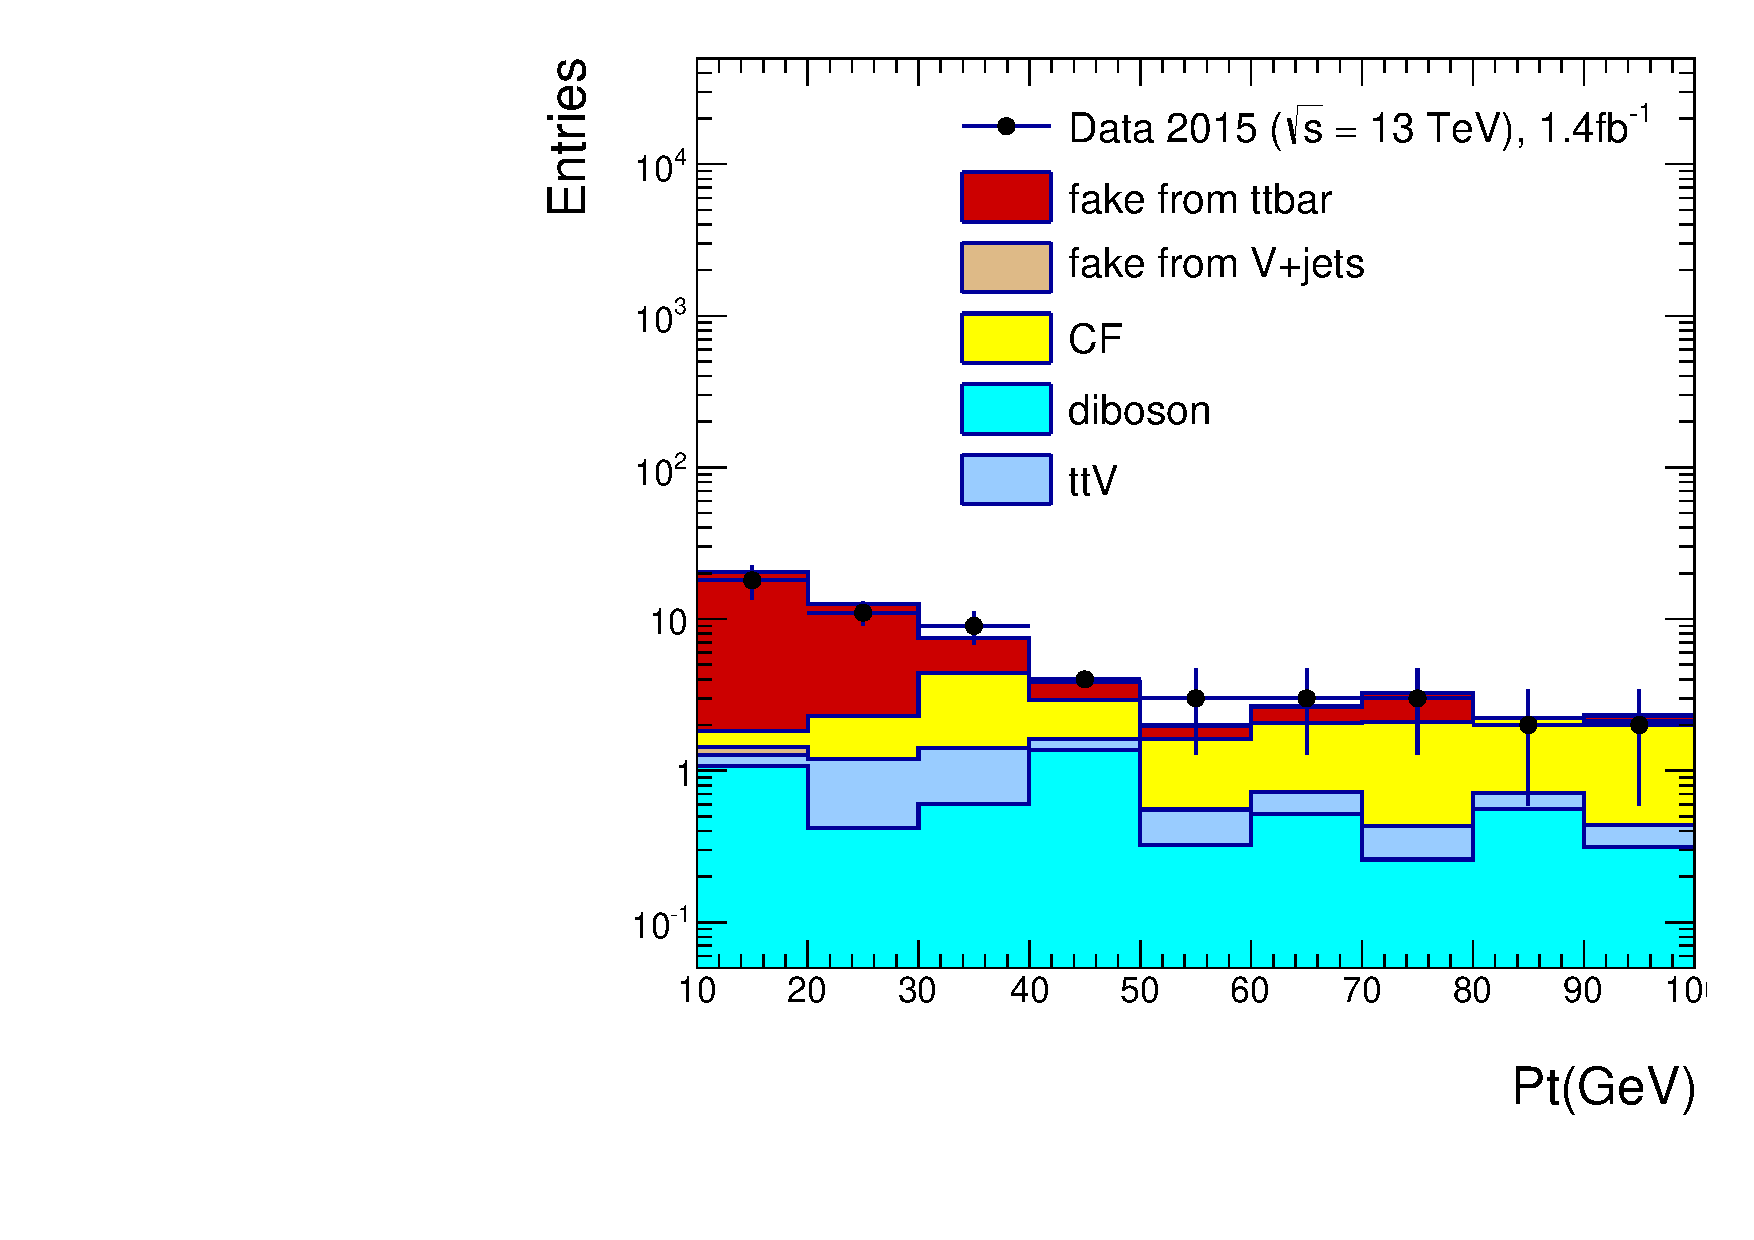
\includegraphics[width=0.49\textwidth]{BKG/fakeEff/el_signal.pdf}
}
\caption
{Probe electron \pt distribution in data and MC.}
\label{Fig:CR_fake_ele}
\end{figure}
%%

%
\begin{table}
\centering
%\resizebox{\textwidth}{!}{
\begin{tabular}{|c|c|c|} \hline
Samples & $10 <p_T<20$ \GeV\ & $p_T > 20$\GeV\ \\ \hline  \hline
\multicolumn{3}{|c|}{Events with a tight probe electron}  \\ \hline
Data & $33.00$ & $39.00$  \\ \hline
Multi-boson & $0.60 \pm 0.14$ & $1.73 \pm 0.30$  \\
$\ttbar+W/Z$ & $0.42 \pm 0.04$ & $3.14 \pm 0.10$  \\
Other & $0.26 \pm 0.06$ & $1.30 \pm 0.14$  \\
Charge flip & $1.26 \pm 0.05 \pm 0.88$ & $11.02 \pm 0.31 \pm 1.73$  \\ \hline  \hline
\multicolumn{3}{|c|}{Events with a loose probe electron}  \\ \hline
Data & $387.00$ & $186.00$  \\ \hline
Multi-boson & $0.68 \pm 0.16$ & $0.99 \pm 0.27$  \\
$\ttbar+W/Z$ & $0.66 \pm 0.05$ & $1.01 \pm 0.06$  \\
Other & $0.50 \pm 0.10$ & $0.51 \pm 0.09$  \\
Charge flip & $12.89 \pm 0.46 \pm 16.16$ & $28.07 \pm 0.93 \pm 4.44$  \\ \hline  \hline
\multicolumn{3}{|c|}{When tag muon fails signal cuts} \\ \hline
Data & $30.00$ & $9.00$  \\ \hline
Multi-boson & $0.12 \pm 0.05$ & $0.06 \pm 0.04$  \\
$\ttbar+W/Z$ & $0.02 \pm 0.01$ & $0.04 \pm 0.01$  \\
Other & $0.03 \pm 0.02$ & $0.01 \pm 0.02$  \\ \hline
\end{tabular}% }
\caption{Number of selected events with a tag muon and a tight/loose probe electron in data and MC, as used for the electron fake rate computation (first two tables), in the presence of at least one b-jet. Only statistical uncertainties are shown, including the uncertainties on the charge flip rates. The third table shows for reference the number of events in which the ``tag'' muon fails the signal requirements.}
\label{table:fake_electron_bjet}
\end{table}
%
\begin{table}
\centering
\begin{tabular}{|c|c|c|} \hline
Sample & $10 <p_T<2$ \GeV\ & $p_T > 20$\GeV\ \\\hline\hline
Data & 0.076 $\pm$ 0.014 $\pm$ 0.038 &  0.123 $\pm$ 0.024 $\pm$ 0.065\\ 
MC   & 0.047 $\pm$  0.001  &  0.042 $\pm$ 0.001 \\\hline 
\end{tabular}
\caption{Measured electron (absolute) fake rate in data and in MC, including the presence of at least one b-jet. The statistical and the systematic uncertainties are displayed for the data measurements, and only the statistical uncertainty for the MC measurements. The results in MC correspond to a luminosity of 3~\ifb.}
\label{table:fake_electron_bjet_Data_MC}
\end{table}


%%
\par{\bf Fake muon efficiency measurement\\}
Same-sign dimuon pairs are used for the measurement in data, similarly to the electron case; 
the criteria for the selection of the tag muon are identical, and it is in addition required to have a larger transverse momentum than the probe muon. 
The measurement can be performed only up to 40~GeV, and above the same value as in the [20, 40]~\GeV \pt bin is used. 
 
The numbers of events with tight and loose probe muons used for the measurement are shown in Table~\ref{table:fake_muon} 
for data and for Monte Carlo (which are used for the prompt SS subtraction). 
Figure~\ref{Fig:CR_fake_mu} shows the $p_T$ distribution of numerator and denominator in data and MC. 
For completeness we choose to show the detector background estimation from \ttbar\ and $V$+jets MC samples. 
Data and MC prediction are in fair agreement and the selection is dominated by $t\bar t$ events. 
The measured muon fake rates (with their statistical uncertainties) are shown in Table~\ref{table:fake_muon_bjet_Data_MC}. 
Both the results in data and in $V$+jets and \ttbar\ MC are shown. A good agreement between the two measurements is obtained. 

%%
\begin{figure}[h!]
\centering
\subfigure[CR$_{1bF}$, baseline probe muon]
{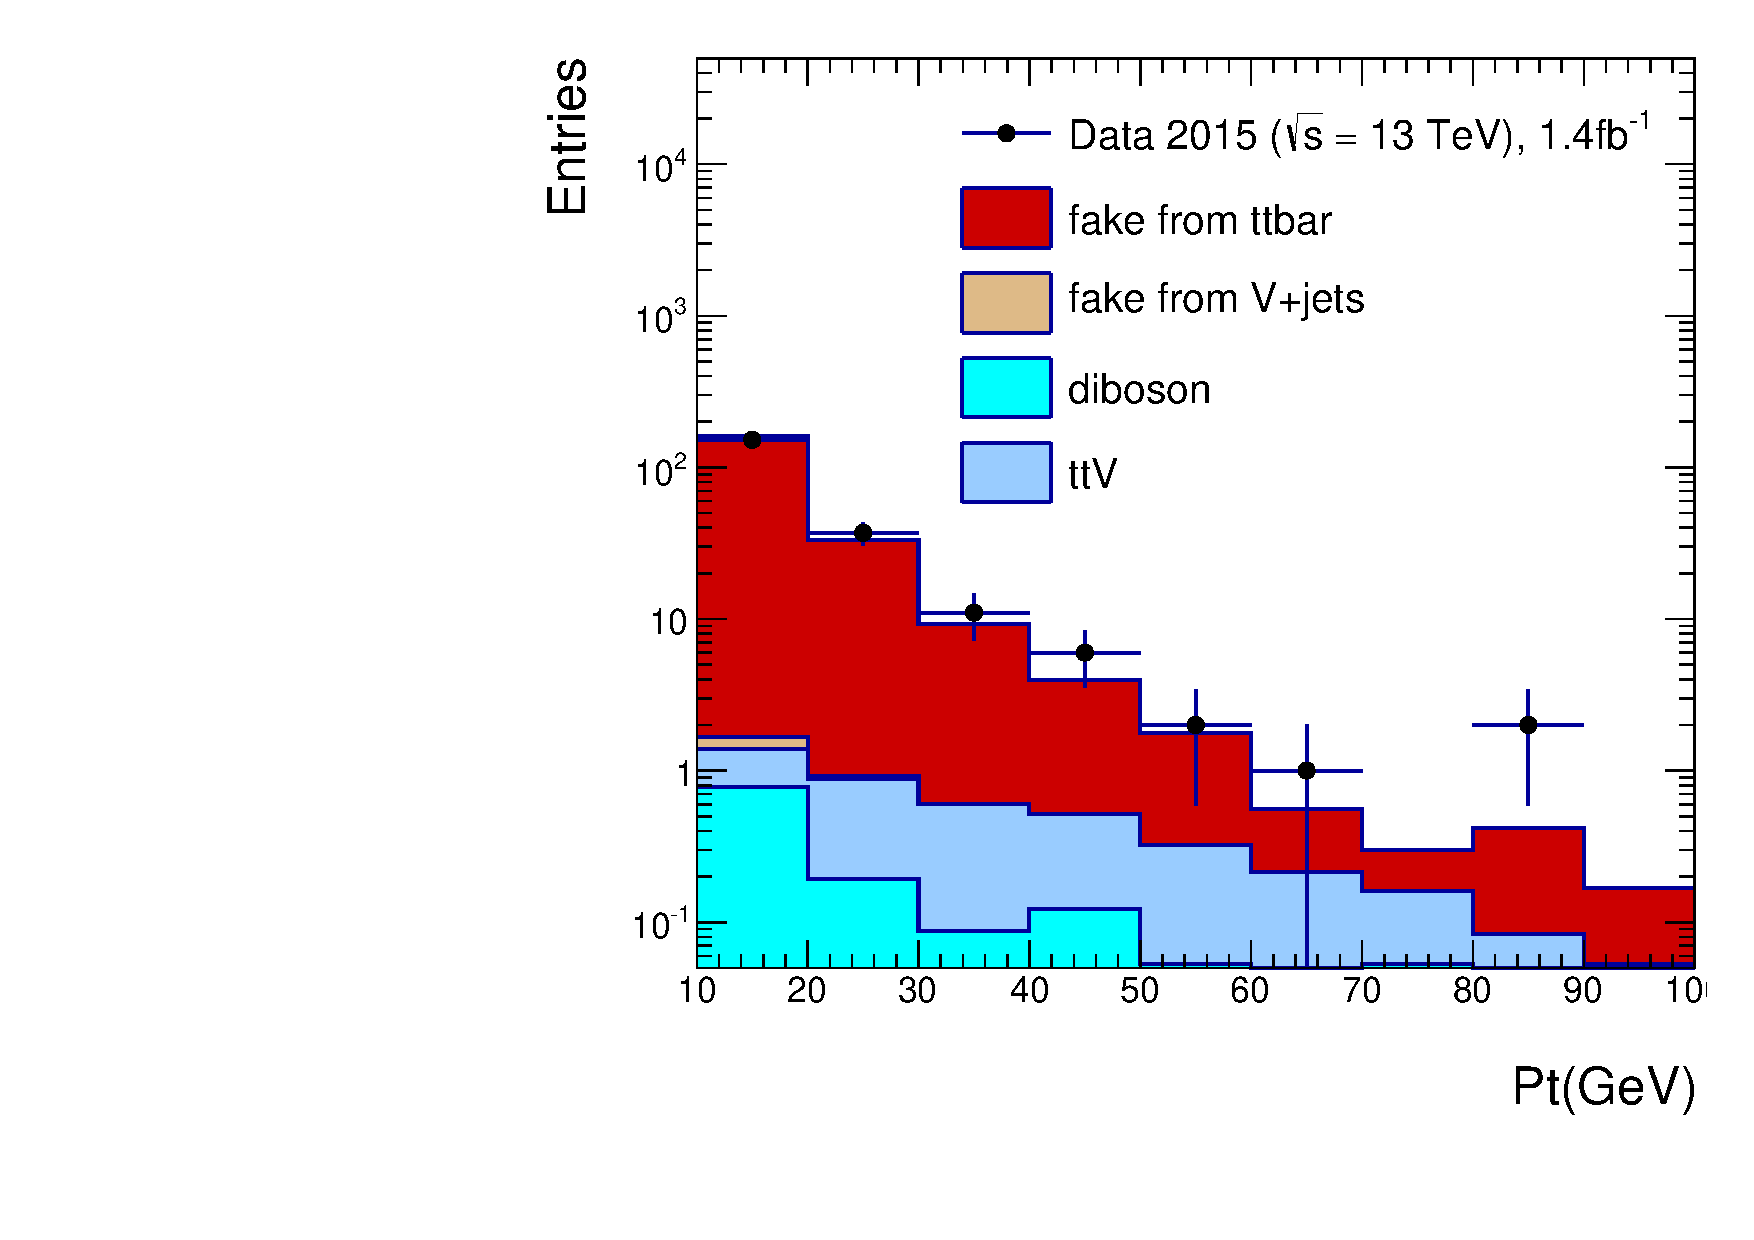
\includegraphics[width=0.49\textwidth]{BKG/fakeEff/mu_baseline.pdf}}
\subfigure[CR$_{1bF}$, signal probe muon]{
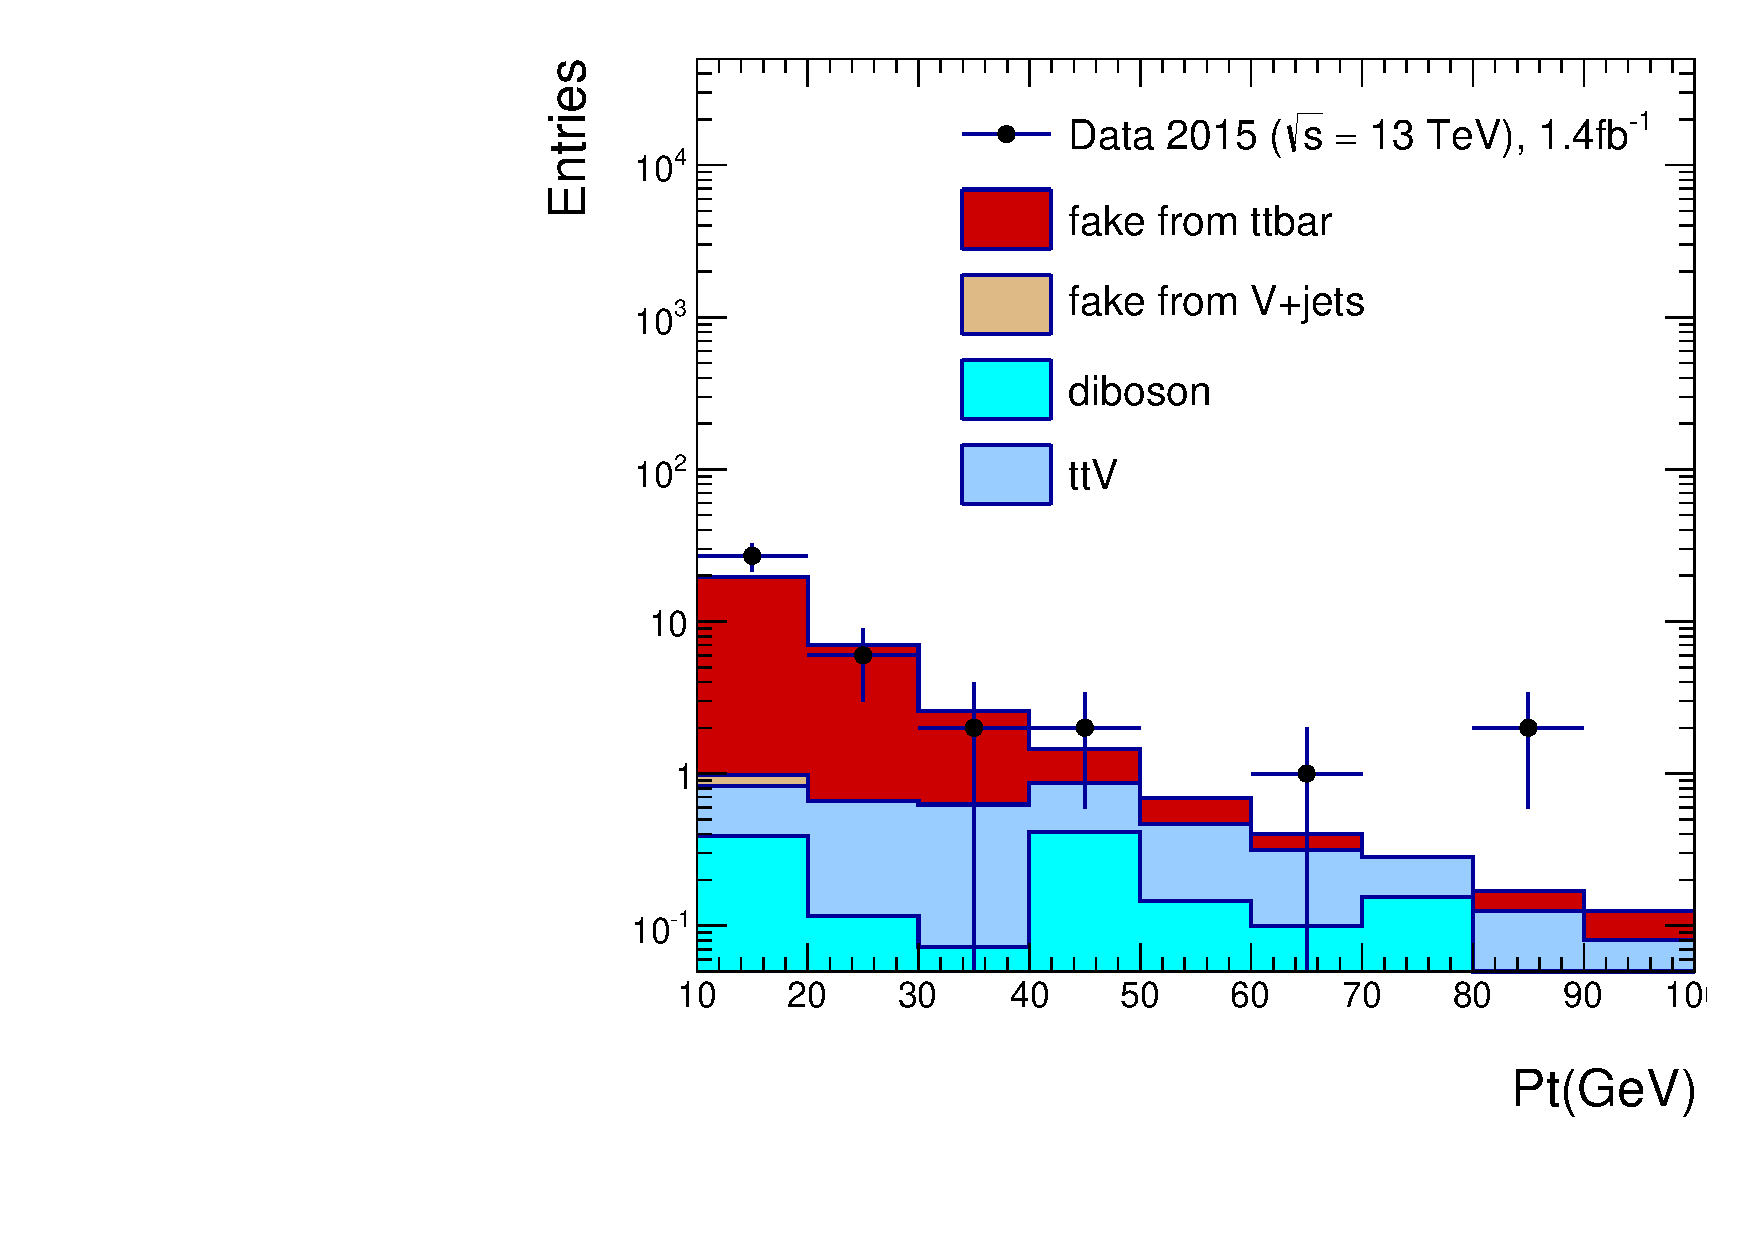
\includegraphics[width=0.49\textwidth]{BKG/fakeEff/mu_signal.pdf}
}
\caption
{Probe muon \pt distribution in data and MC.}
\label{Fig:CR_fake_mu}
\end{figure}
%%


\begin{table}
\centering
\begin{tabular}{|c|c|c|c|} \hline
Samples & $10 <p_T<15$ \GeV\ & $15 <p_T<20$ \GeV\ & $p_T > 20$ \GeV\ \\ \hline  \hline
\multicolumn{4}{|c|}{Events with a tight probe muon}  \\ \hline
Data & $45.00$ & $15.00$ & $18.00$  \\ \hline
Multi-boson & $0.07 \pm 0.17$ & $0.31 \pm 0.11$ & $1.45 \pm 0.23$  \\
$\ttbar+W/Z$ & $0.48 \pm 0.04$ & $0.52 \pm 0.04$ & $2.50 \pm 0.09$  \\
Other & $0.32 \pm 0.07$ & $0.24 \pm 0.07$ & $0.79 \pm 0.12$  \\  \hline \hline
\multicolumn{4}{|c|}{Events with a loose probe muon} \\ \hline
Data & $193.00$ & $92.00$ & $102.00$  \\ \hline
Multi-boson & $0.69 \pm 0.19$ & $0.31 \pm 0.10$ & $0.70 \pm 0.20$  \\
$\ttbar+W/Z$ & $0.27 \pm 0.03$ & $0.20 \pm 0.03$ & $0.42 \pm 0.04$  \\
Other & $0.32 \pm 0.07$ & $0.31 \pm 0.06$ & $0.30 \pm 0.06$  \\ \hline  \hline
\multicolumn{4}{|c|}{When tag muon fails signal cuts} \\ \hline
Data & $6.00$ & $2.00$ & $5.00$  \\ \hline
Multi-boson & $0.08 \pm 0.06$ & $0.03 \pm 0.03$ & $-0.05 \pm 0.05$  \\
$\ttbar+W/Z$ & $0.01 \pm 0.01$ & $0.01 \pm 0.01$ & $0.04 \pm 0.01$  \\
Other & $0.01 \pm 0.01$ & $0.00 \pm 0.00$ & $0.07 \pm 0.03$  \\ \hline
\end{tabular}
\caption{Number of selected events with a tag muon and a tight/loose probe muon in data and MC, as used for the muon fake rate computation (first two tables), in the presence of at least one b-jet. Only statistical uncertainties are shown, including the uncertainties on the charge flip rates. The third table shows for reference the number of events in which the ``tag'' muon fails the signal requirements, 
but in that case numbers are biased since the tag muon is matched to a trigger requiring an isolated muon.}
\label{table:fake_muon}
\end{table}
%
\begin{table}
\centering
\begin{tabular}{|c|c|c|c|} \hline
Sample & $10 <p_T<15$ \GeV\ & $15 <p_T<20$ \GeV\ & $p_T > 20$\GeV\ \\\hline\hline
Data &0.187 $\pm$ 0.026 $\pm$ 0.094 & 0.133 $\pm$ 0.034 $\pm$ 0.066 & 0.116 $\pm$ 0.035 $\pm$ 0.059 \\ 
MC   &0.131 $\pm$ 0.002 & 0.103 $\pm$ 0.002 & 0.113 $\pm$ 0.002 \\\hline 
\end{tabular}
\caption{Measured muon fake rate in data and in MC, including the presence of at least one b-jet. The statistical and the systematic uncertainties are displayed for the data measurements, and only the statistical uncertainty for the MC measurements. The results in MC correspond to a luminosity of 3~\ifb.}
\label{table:fake_muon_bjet_Data_MC}
\end{table}

%%
%\par{\bf Fake rate for very energetic leptons\\}
%The lepton fake rate at hight \pt (as high as 100 - 200~GeV) cannot be studied in data or in any of the Monte Carlo samples available for the Standard Model processes, 
%given the very low available statistics. 
%Therefore, we investigate the energetic fake leptons using SUSY signal samples (gluino pair production via on- and off-shell squarks, direct sbottom pair production, etc). 
%The composition in a region with at least one $b$-jet is found to be similar as in the signal regions. 
%The results are shown in Figure~\ref{Fig:Fake_Rate_HighPt} for electrons (left) and muons (right). 
%Generally, the fake rate is not found to significantly increase at high \pt. 
%The difference with respect to the fake rate measured at low \pt (as used in the analysis)  is within the assigned systematic uncertainty. 

 
%\begin{figure}[h!]
%\centering
%\subfigure{
%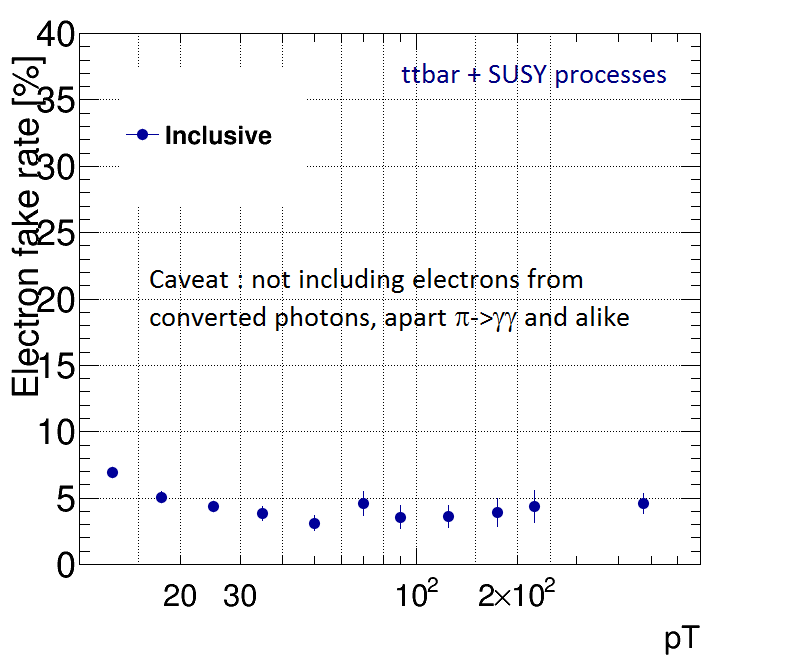
\includegraphics[width=0.45\textwidth]{BKG/fakeEff/FakeRate_HighPT/Var2_FakeEL_Reg_Incl_EM_EE_pt}
%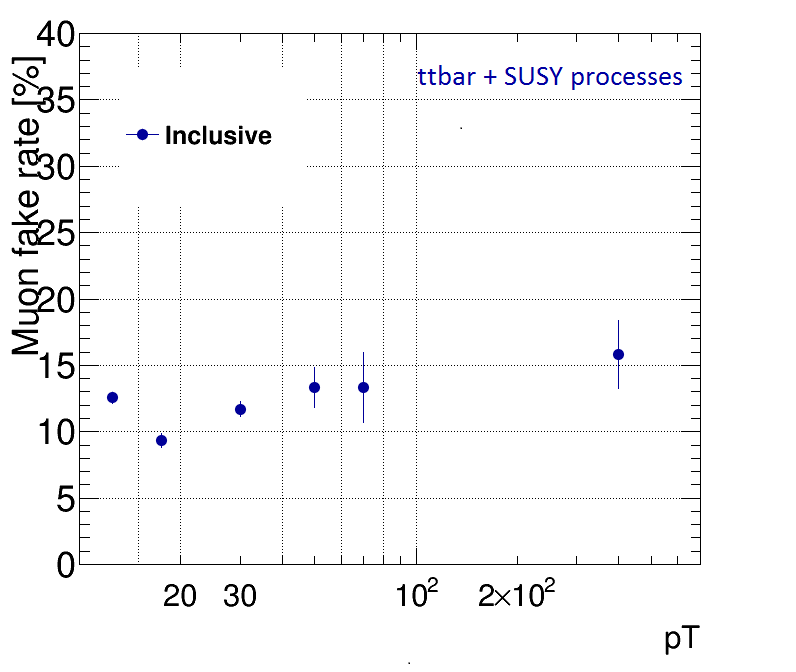
\includegraphics[width=0.45\textwidth]{BKG/fakeEff/FakeRate_HighPT/Var2_FakeMU_Reg_Incl_EM_MM_pt}
%}
%\vspace{-0.2cm}
%\caption{Electron (left) and muon (right) fake rate for very energetic leptons in MC. Only the statistical uncertainties are shown. [Plots to be updated!]}
%\label{Fig:Fake_Rate_HighPt}  
%\end{figure} 

%%
\par{\bf Corrections for regions with two or three $b$-jets\\}
In \ttbar\ events, the fake lepton might have less chances to come from a $B$-meson decay if there are already 2 tagged jets (section~\ref{sec:truthComposition_SR}). 
As the fake rate changes between a region with 1 $b$-jet or 2 $b$-jets, 
we chose to study the fake rate separately in regions with at least 1, 2 and 3 $b$-jets in $V$+jets and \ttbar\ MC, 
and in data when the statistic allows us. 
The results in MC are shown in Figure~\ref{Fig:Fake_Rate_nbJets} for electrons (left) and for muons (right). 
The fake rate is found to have a variation of $O$(30\%). 
The fake rate measured in data in a region with $\geq$2 $b$-jets is found to be consistent with the rate measured $\geq$1 $b$-jet 
-- large statistical uncertainties are obtained. 
All results are shown in Table~\ref{table:fake_muon_nrbjets_Data_MC} . 
  
\begin{figure}[h!]
\centering
\subfigure{
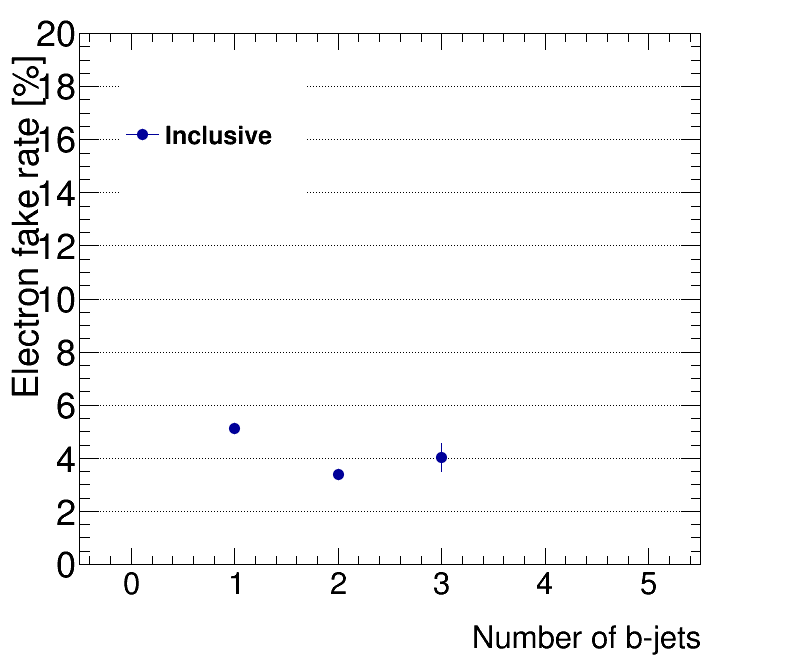
\includegraphics[width=0.45\textwidth]{BKG/fakeEff/FakeRate_MC/Var2_FakeEL_Reg_Incl_EM_EE_nbJets}
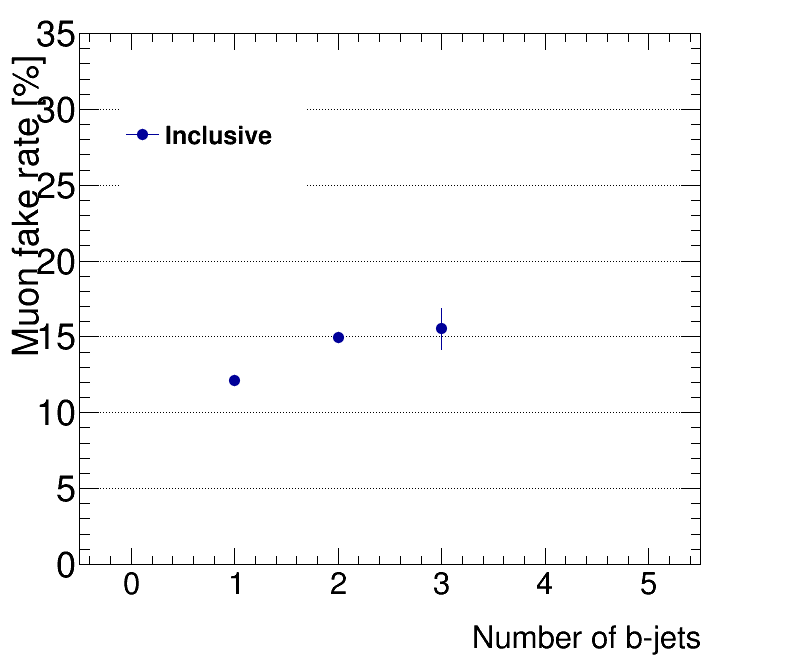
\includegraphics[width=0.45\textwidth]{BKG/fakeEff/FakeRate_MC/Var2_FakeMU_Reg_Incl_EM_MM_nbJets}
}   
\vspace{-0.2cm}
\caption{Electron (left) and muon (right) fake rate in Monte-Carlo as a function of number of $b$-jets in the event. 
Only the statistical uncertainties are shown. $L$=3~\ifb.}
\label{Fig:Fake_Rate_nbJets}  
\end{figure}
%%
%
\begin{table}
\centering
\begin{tabular}{|c|c|c|c|} \hline
Sample & $\geq$1 $b$-jet & $\geq$2 $b$-jets & $\geq$3 $b$-jets \\\hline\hline  
\multicolumn{4}{|c|}{Electron fake rate} \\ \hline
Data & 0.079 $\pm$ 0.014 & 0.09 $\pm$ 0.034 & -\\ 
MC   &0.051 $\pm$ 0.001 & 0.034 $\pm$ 0.001 & 0.040 $\pm$0.005\\\hline  \hline
\multicolumn{4}{|c|}{Muon fake rate} \\ \hline
Data &0.150 $\pm$ 0.018 & 0.194 $\pm$ 0.067 & -\\ 
MC   &0.121 $\pm$ 0.002 & 0.149 $\pm$ 0.003 &0.155 $\pm$ 0.014 \\\hline 
\end{tabular}  
\caption{Muon fake rate in data and in MC, as a function of number of $b$-jets in the event. 
Only the statistical uncertainty is displayed. The results in MC correspond to a luminosity of 3~\ifb.}
\label{table:fake_muon_nrbjets_Data_MC}
\end{table}


%%
\par{\bf Dependency to other kinematic variables\\}
In data we don't have enough statistics to performed a binned measurement in $\Delta R$, number of jets in the events, \met, $\eta$, etc. 
Therefore, we check the possible dependencies of the lepton fake efficiencies to other variables in $V$+jets and \ttbar\ MC. 
The obtained results are shown in Figure~\ref{Fig:Fake_Rate_ELE_Variations} for electrons and in Figure~\ref{Fig:Fake_Rate_MU_Variations} for muons. 
The strongest variations are seen for the muon fake rate, that increases steadily with $p_T$. 
The other variations are within the uncertainties assigned to the fake rate (see below). 

\begin{figure}[hp!]
\centering
\subfigure{
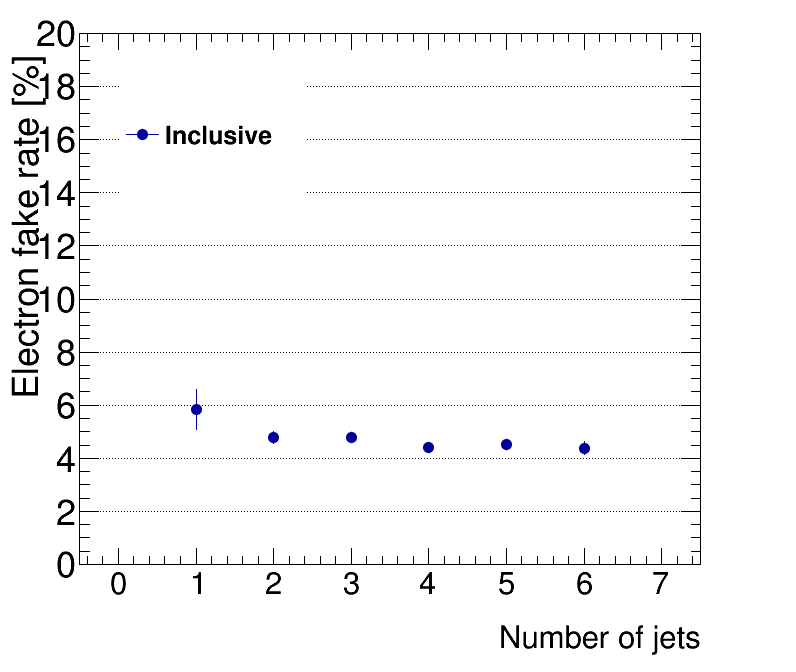
\includegraphics[width=0.45\textwidth]{BKG/fakeEff/FakeRate_MC/Var2_FakeEL_Reg_Incl_EM_EE_nJets}
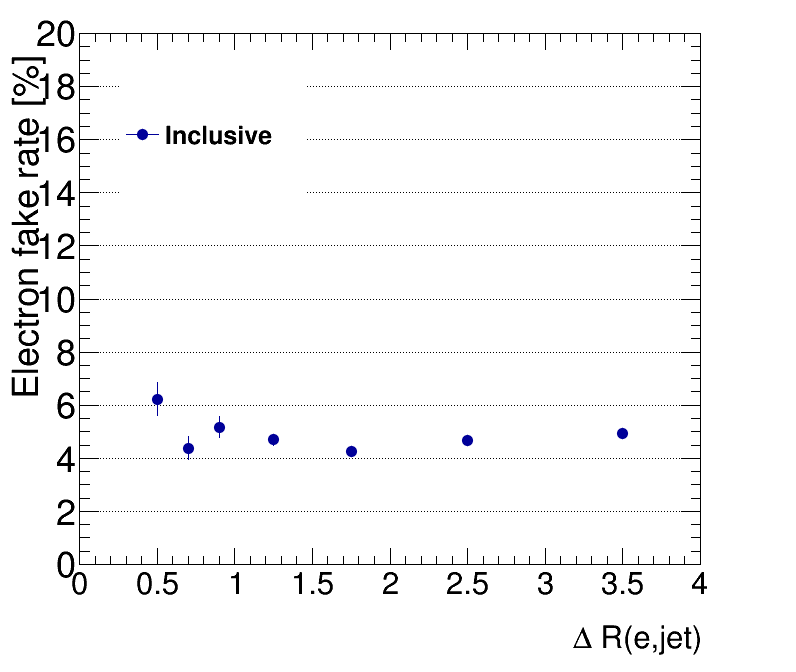
\includegraphics[width=0.45\textwidth]{BKG/fakeEff/FakeRate_MC/Var2_FakeEL_Reg_Incl_EM_EE_dr}
}   
\subfigure{
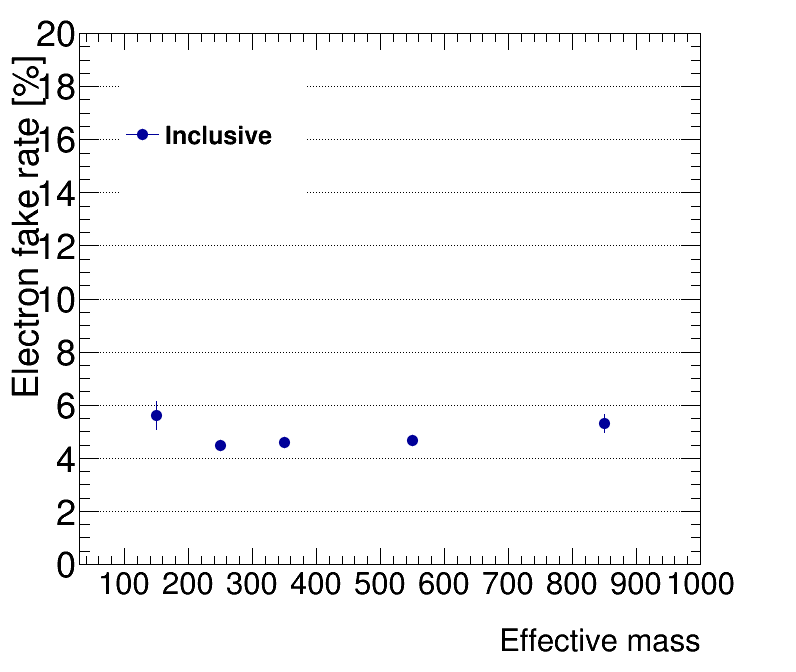
\includegraphics[width=0.45\textwidth]{BKG/fakeEff/FakeRate_MC/Var2_FakeEL_Reg_Incl_EM_EE_meff}
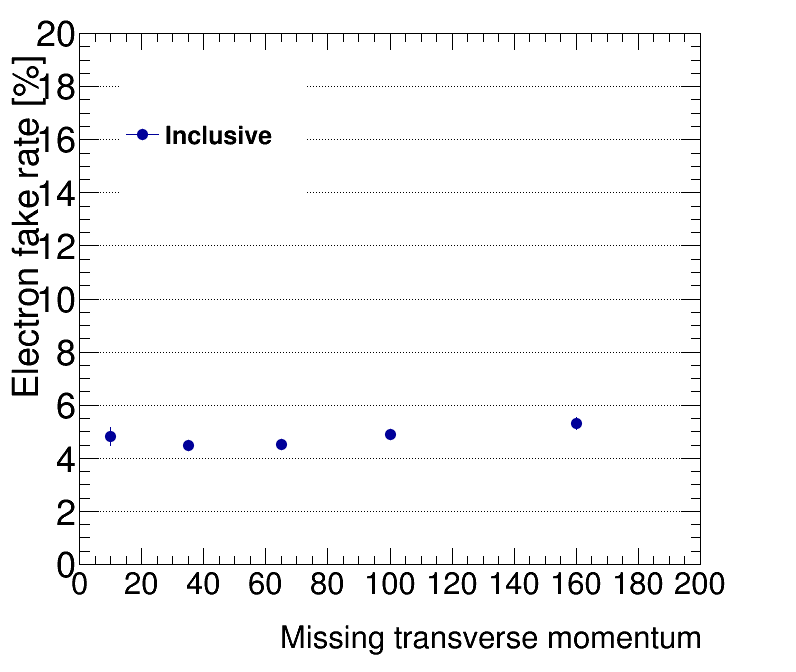
\includegraphics[width=0.45\textwidth]{BKG/fakeEff/FakeRate_MC/Var2_FakeEL_Reg_Incl_EM_EE_met}
}   
\subfigure{
\includegraphics[width=0.45\textwidth]{BKG/fakeEff/FakeRate_MC/Var2_FakeEL_Reg_Incl_EM_EE_pt}
\includegraphics[width=0.45\textwidth]{BKG/fakeEff/FakeRate_MC/Var2_FakeEL_Reg_Incl_EM_EE_eta}
}
\vspace{-0.2cm}
\caption{Electron fake rate in Monte-Carlo as a function of number of number of jets and $\Delta R(l, jet)$ (top), \meff\ and \met\ (middle), and \pt and $\eta$ (bottom) variables. Only the statistical uncertainties are shown. $L$=3~\ifb.}
\label{Fig:Fake_Rate_ELE_Variations}  
\end{figure}
%%
\begin{figure}[hp!]
\centering
\subfigure{
\includegraphics[width=0.45\textwidth]{BKG/fakeEff/FakeRate_MC/Var2_FakeMU_Reg_Incl_EM_MM_nJets}
\includegraphics[width=0.45\textwidth]{BKG/fakeEff/FakeRate_MC/Var2_FakeMU_Reg_Incl_EM_MM_dr}
}   
\subfigure{
\includegraphics[width=0.45\textwidth]{BKG/fakeEff/FakeRate_MC/Var2_FakeMU_Reg_Incl_EM_MM_meff}
\includegraphics[width=0.45\textwidth]{BKG/fakeEff/FakeRate_MC/Var2_FakeMU_Reg_Incl_EM_MM_met}
}   
\subfigure{
\includegraphics[width=0.45\textwidth]{BKG/fakeEff/FakeRate_MC/Var2_FakeMU_Reg_Incl_EM_MM_pt}
\includegraphics[width=0.45\textwidth]{BKG/fakeEff/FakeRate_MC/Var2_FakeMU_Reg_Incl_EM_MM_eta}
}
\vspace{-0.2cm}
\caption{Muon fake rate in Monte-Carlo as a function of number of number of jets and $\Delta R(l, jet)$ (top), \meff\ and \met\ (middle), and \pt and $\eta$ (bottom) variables. Only the statistical uncertainties are shown. $L$=3~\ifb.}
\label{Fig:Fake_Rate_MU_Variations}  
\end{figure}
%%


%%
\par{\bf Systematic uncertainties\\}
The measurements of fake leptons efficiencies are associated to large uncertainties which cover the nature of the fake leptons 
and the events that produce them being different between the measurement and signal regions. 
In this analysis several sources of systematic uncertainties are considered : 
\begin{itemize}
	\item{Uncertainty due to the subtraction of prompt leptons processes in the measurement region: 
	it is assigned by varying the MC normalizations by 30$\%$, 
	to cover the uncertainty on the production cross section, MC statistics, etc.}
	\item{Fake rate evolution with $p_T$: while Fig.~\ref{Fig:Fake_Rate_MU_Variations} shows a significant increase of the muon fake rate with $p_T$, 
	the MC predictions suggest that the yield of high $p_T$ fake leptons should be negligible in the signal regions (see e.g. Fig~\ref{Fig:Fake_Composition_CR}). 
	By lack of time and statistics in data, we do not address this dependency, 
	and observe that the uncertainty assigned below therefore resonably covers the observed variations for fake leptons up to $p_T=40$ GeV 
	(Fig.~\ref{Fig:Fake_Rate_ELE_Variations} and~\ref{Fig:Fake_Rate_MU_Variations}) -- and trusting the MC indications that higher $p_T$ fakes are not a concern.}
	\item{Lepton fake rate in regions with 2-3 b jets: $O(30\%)$ the relative difference between the fake rate measured with $\geq$1 $b$-jet and with $\geq$2-3 $b$-jets in MC.}
	\item{Dependency on other kinematic variables: $O(30\%)$ for both electrons and muons.}	
	%\item{Changes in the sample composition: plan to design complementary control regions to measure the fake rate in data. Not done yet (need more data).}
\end{itemize}

To cover all these sources of systematic uncertainties, we choose to apply an overall systematic uncertainty of 50\% on the fake rates treated as uncorrelated between the different bins.

A Monte-Carlo closure test is performed to validate the measurement of the lepton fake rate and electron charge-flip rate, as documented in Appendix~\ref{app:ClosureTest}.
